\documentclass[10pt,letterpaper,final]{article}

% Paquetes
\usepackage[utf8]{inputenc}
\usepackage[spanish]{babel}
\usepackage{amsmath}
\usepackage{graphicx}
\usepackage{hyperref}
\usepackage{tocbibind} % Para incluir referencias en el índice
\usepackage{caption}
\usepackage{subcaption} % Paquete para justificar el texto

% Información del documento
\title{Estimación de la pose de un vehículo mediante cámaras y sensores para estacionamiento automático en simulación}
\author{Ing. Rubén Martínez González}
\date{Septiembre 2025}
\newcommand{\university}{Universidad Autónoma de Yucatán}
\newcommand{\faculty}{Facultad de Matemáticas}
\newcommand{\advisor}{Dr. Arturo Espinosa Romero}
\newcommand{\myauthor}{Ing. Rubén Martínez González}
\newcommand{\degree}{Maestría en Ciencias de la Computación}
\newcommand{\tesisInv}{Tesis de investigación}
\newcommand{\mydate}{Septiembre 2025}
\newcommand{\mytitle}{Estimación de la pose de un vehículo mediante cámaras y sensores para estacionamiento automático en simulación}

\begin{document}

% Portada moderna
\begin{titlepage}
    \centering
    % Logos
    \begin{minipage}{0.25\textwidth}
        \centering
        
\includegraphics[width=0.8\textwidth]{img/fmat.png}
    \end{minipage}%
    \hfill
    \begin{minipage}{0.5\textwidth}
        \centering
        {\scshape\small \university \par}
        \vspace{0.2cm}
        {\scshape\small \faculty \par}
        \vspace{0.2cm}
        {\scshape\small \degree \par}
    \end{minipage}%
    \hfill
    \begin{minipage}{0.25\textwidth}
        \centering
        
\includegraphics[width=0.8\textwidth]{img/UADY.jpg}
    \end{minipage}

    \vspace{1.5cm}
    {\LARGE\bfseries \mytitle \par}
    \vspace{1.5cm}
    {\Large \tesisInv \par}
    \vspace{1cm}
    {\large Autor: \textbf{\myauthor}\par}
    \vspace{0.5cm}
    {\large Asesor: \textbf{\advisor}\par}
    \vfill
    \vspace{0.5cm}
    {\large \mydate \par}
\end{titlepage}

% Resumen
\begin{abstract}
    \noindent
Este documento presenta un enfoque para la estimación de la posición de un vehículo en un entorno de estacionamiento
utilizando técnicas de visión por computadora y aprendizaje automático. Se describe la implementación de un sistema
de simulación que permite la recolección de datos de sensores y la generación de imágenes sintéticas para entrenar 
modelos de detección de objetos. Los resultados muestran la efectividad del enfoque propuesto en la identificación de 
espacios de estacionamiento y la navegación autónoma en entornos complejos.
\end{abstract}
\clearpage


% Índice
\tableofcontents
\listoffigures
\clearpage

% Capítulo 1: Introducción
\section{Introducción}
\noindent
El estacionamiento es una actividad esencial en la vida urbana, ya que permite a los conductores dejar sus vehículos en reposo mientras realizan otras actividades.
No obstante, el estacionamiento en áreas urbanas congestionadas presenta múltiples desafíos, incluyendo la falta de espacio,
la presencia de obstáculos y la visibilidad reducida, lo cual incrementa el riesgo de colisiones y daños a los vehículos.
Incluso habiendo identificado el espacio de estacionamiento, el proceso de maniobrar el vehículo para estacionar puede ser complicado y estresante,
especialmente para conductores con poca experiencia o en vehículos grandes.\\
\noindent
Para mitigar estos problemas, se han desarrollado sistemas avanzados de asistencia al conductor, como el estacionamiento automático,
que facilitan esta tarea y mejoran la seguridad.
Sin embargo, la efectividad de estos sistemas depende en gran medida de la capacidad para estimar con precisión la posición del vehículo
con respecto al espacio de estacionamiento.
Una estimación incorrecta puede resultar en maniobras inseguras, especialmente en entornos con espacio limitado.\\
\noindent
Representar esta ubicación de manera adecuada es crucial para el desarrollo de un sistema de estacionamiento automático confiable.
Para abordar esta cuestión, se propone diseñar una simulación en donde se obtendrán datos de sensores
y cámaras del vehículo para estimar su posición relativa al espacio de estacionamiento.\\
\noindent
La simulación se llevará a cabo en un entorno controlado que refleja las condiciones reales de estacionamiento.
%Se modelará un escenario de estacionamiento con un vehículo y su espacio de estacionamiento, donde se adquirirán datos de sensores.
Dicho entorno consistirá de un cajón de estacionamiento objetivo, el vehículo que se va a controlar y objetos estáticos que pueden generar oclusiones.
El entorno de simulación permitirá extraer información a través de sensores los cuales permitirán hacer mediciones de las distancias y ángulos necesarios para maniobrar durante el estacionamiento.\\
\noindent
Las mediciones obtenidas, representadas mediante coordenadas cilíndricas, proporcionarán la información necesaria para entrenar algoritmos de aprendizaje automático.
Estos algoritmos podrán aprender y adaptarse a diversas condiciones y escenarios, mejorando la precisión y seguridad del sistema de estacionamiento automático.\\
\noindent
La investigación se centra en desarrollar un sistema que, mediante la estimación de la posición del vehículo y la simulación de este entorno, permita avanzar en la creación de sistemas de estacionamiento automático eficientes y seguros en entornos urbanos congestionados.

\subsection{Contexto y problemática}
\noindent
%    problemas en los estacionamientos
Los estacionamientos son imprescindibles en la vía urbana, ya que permiten a los conductores estacionar sus vehículos
de manera segura y eficiente. Sin embargo, el proceso de estacionamiento puede ser complicado y estresante,
especialmente en áreas congestionadas con espacio limitado y visibilidad reducida.
Factores como la falta de espacio, la presencia de obstáculos y la poca visibilidad para el conductor ocasionan
dificultades al estacionar un vehículo, lo que puede aumentar el riesgo de colisiones y daños al vehículo.
\\
%   se han logrado sistemas de asistencia al conductor
En la actualidad, la búsqueda de soluciones para mejorar la eficiencia y seguridad en el desplazamiento vehicular
ha llevado al desarrollo de sistemas avanzados de asistencia al conductor.
Entre estos sistemas, el estacionamiento automático ha ganado relevancia como una función que puede contribuir
a reducir los riesgos asociados con el estacionamiento en entornos urbanos congestionados.
\\
%   problemas de sistemas de estacionamiento automático
Sin embargo, el desarrollo de sistemas de estacionamiento automático presenta desafíos significativos,
especialmente en lo que respecta a la estimación de la posición del vehículo con respecto al espacio de estacionamiento.
El cálculo incorrecto de esta posición puede resultar en maniobras de estacionamiento inseguras o peligrosas,
especialmente en entornos donde el espacio de estacionamiento es limitado o con poca visibilidad para el conductor.
\\
%   necesidad de sistemas de asistencia al conductor más autónomos
En este contexto, continua la necesidad de desarrollar soluciones de utilidad para que los sistemas de asistencia al conductor
sean cada vez más autosuficientes y no dependan de la intervención limitada del conductor.
\\
%   en que consiste la investigación
Esta investigación se enfoca en poder estimar la posición de un vehículo con respecto a su espacio de estacionamiento
utilizando cámaras y sensores y utilizar esta posición estimada para lograr un sistema de estacionamiento automático en simulación.

\subsection{Preguntas de investigación}

\begin{itemize}
    \item ¿Cómo se puede representar la posición de un vehículo con respecto a su espacio de estacionamiento?
    \item ¿Cómo se puede estimar esta posición utilizando las cámaras y sensores del vehículo?
    \item ¿Cómo usar esta posición estimada para que el vehículo se estacione automáticamente?
\end{itemize}

\subsection{Hipótesis}
\noindent
``Estimando la posición relativa al estacionamiento de un vehículo mediante cámaras y sensores,
y utilizando esta posición, se puede lograr un sistema de estacionamiento automático en simulación.''


\subsection{Objetivos}
\subsubsection{Objetivo General}
\noindent
Desarrollar un sistema de estimación de la posición relativa al estacionamiento de un vehículo mediante cámaras y sensores para estacionamiento automático.

\subsubsection{Objetivos específicos}
\noindent
\begin{itemize}
    \item Modelar un ambiente de simulación de un vehículo y estacionamiento.
    \item Obtener datos de los sensores del vehículo en simulación.
    \item Interpretar los datos de los sensores mediante técnicas de visión computacional.
    \item Procesar los datos y estimar la posición del vehículo con respecto al estacionamiento.
    \item Utilizar la posición estimada para lograr un sistema de estacionamiento automático en simulación.
\end{itemize}

\subsection{Estado del arte - Trabajos previos relacionados}
\noindent\textbf{Autonomous Driving Architectures: Insights of Machine Learning and Deep Learning Algorithms}~\cite{bachute2021autonomous}
El artículo fue publicado en la revista Machine Learning with Applications en 2021 y
proporciona una visión general de la aplicación de algoritmos de Aprendizaje Automático y Aprendizaje Profundo
en sistemas de conducción autónoma, destacando su evaluación en tareas cruciales.
Se destaca el creciente impulso en la investigación de la conducción autónoma debido a sus ventajas inherentes, como la reducción
de la intervención humana y la disociación del conductor del vehículo.
Se subraya la complejidad de estos sistemas,
que involucra la integración de múltiples subsistemas, y se analizan diversas tareas específicas dentro de la conducción autónoma,
como la planificación de movimiento, la detección de peatones y señales de tráfico, el estacionamiento automatizado, entre otras.
El estudio se centra en la aplicación de algoritmos de Aprendizaje Automático y Aprendizaje Profundo para abordar estas tareas,
evaluando y comparando su rendimiento a través de métricas específicas. La investigación ofrece una perspectiva amplia sobre el uso
y la evaluación en el contexto de la conducción autónoma.
\begin{figure}[!ht]
    \centering
    \begin{subfigure}{0.4\textwidth}
        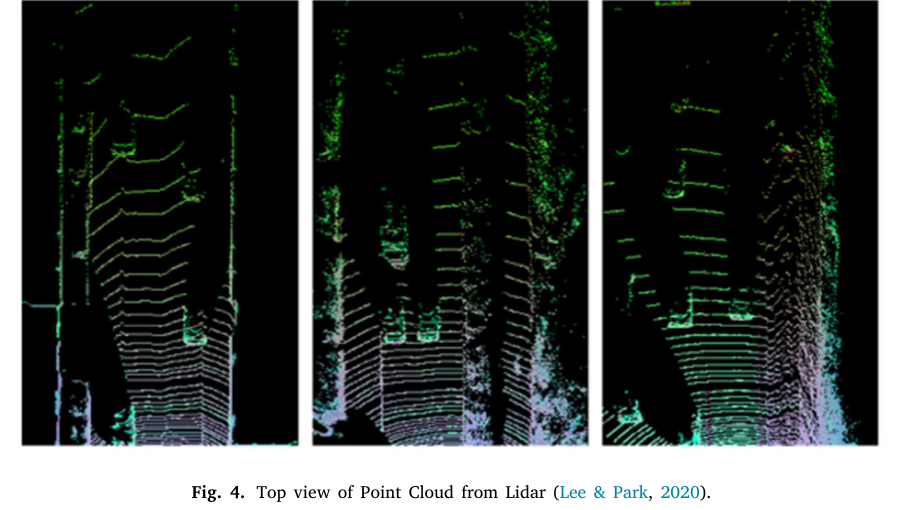
\includegraphics[width=\textwidth]{img/12Screenshot_20231106_142954}\label{fig:12}
    \end{subfigure}
    \begin{subfigure}{0.4\textwidth}
        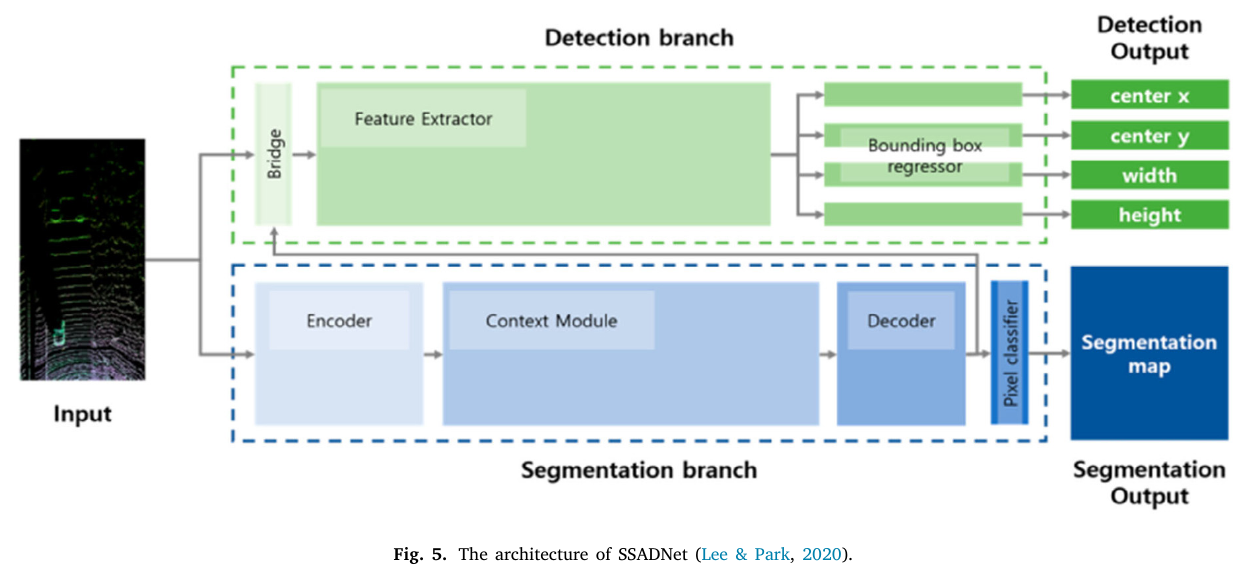
\includegraphics[width=\textwidth]{img/13Screenshot_20231106_143018}\label{fig:13}
    \end{subfigure}
    \begin{subfigure}{0.4\textwidth}
        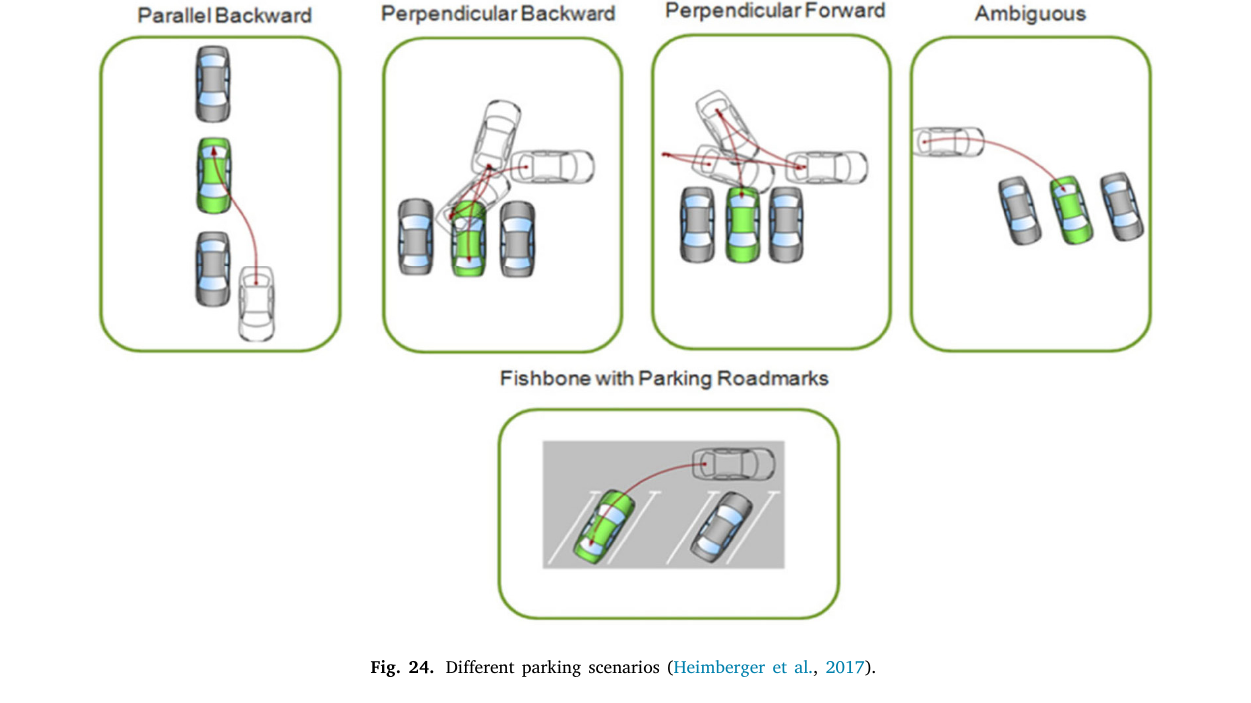
\includegraphics[width=\textwidth]{img/15Screenshot_20231106_143633}\label{fig:15}
    \end{subfigure}
    \begin{subfigure}{0.5\textwidth}
        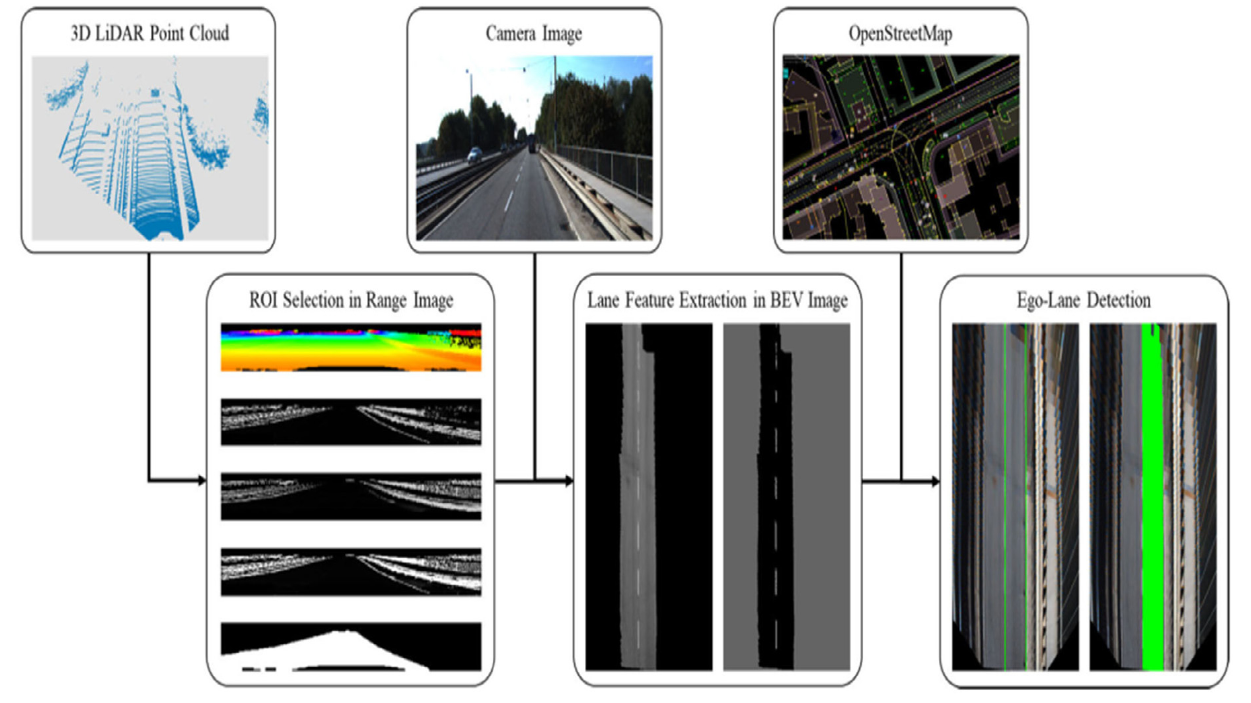
\includegraphics[width=\textwidth]{img/14 Screenshot_20231106_143419}\label{fig:14}
    \end{subfigure}
    \begin{subfigure}{\textwidth}
        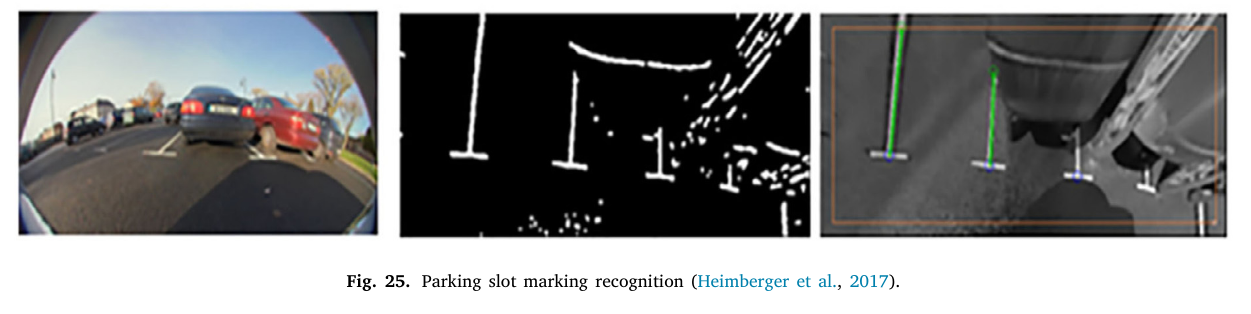
\includegraphics[width=0.99\textwidth]{img/16Screenshot_20231106_143701}\label{fig:16}
    \end{subfigure}
\end{figure}
\clearpage

\noindent\textbf{Vision-based autonomous car racing using deep imitative reinforcement learning}~\cite{cai2021vision}
El artículo fue publicado en la revista IEEE Robotics and Automation Letters en 2021 y aborda el desafío del automovilismo autónomo
en el campo del control robótico, históricamente dependiente de mapas precisos, localización y planificación, lo que lo hace
computacionalmente ineficiente y sensible a cambios en el entorno.
\\
Se destaca el desarrollo de sistemas de aprendizaje profundo de extremo a extremo, que muestran resultados prometedores en la conducción
autónoma.
\\
Sin embargo, estos sistemas suelen basarse en aprendizaje por imitación supervisada (IL), enfrentando problemas de discrepancia
en la distribución de datos.
\\
Aunque se han empleado métodos de aprendizaje por refuerzo (RL), requieren grandes cantidades de datos de interacción riesgosa.
\\
El artículo presenta un enfoque innovador denominado aprendizaje profundo imitativo y de refuerzo (DIRL), que logra la agilidad en
el automovilismo autónomo mediante el uso de entradas visuales.
\\
Este enfoque combina el conocimiento adquirido tanto del aprendizaje por imitación como del aprendizaje basado en modelos de RL,
permitiendo al agente aprender de instructores humanos y mejorar su rendimiento interactuando con un modelo de mundo offline.
La validación del algoritmo se lleva a cabo tanto en simulaciones de conducción de alta fidelidad como en un automóvil RC a escala 1/20 en
el mundo real, con capacidad computacional limitada. \\
Los resultados de la evaluación demuestran que este método supera a enfoques anteriores de IL y RL en eficiencia de muestra y rendimiento
en la tarea, mostrando un gran potencial en el ámbito de la conducción autónoma.
\begin{figure}[!ht]
    \centering
    \begin{subfigure}{0.4\textwidth}
        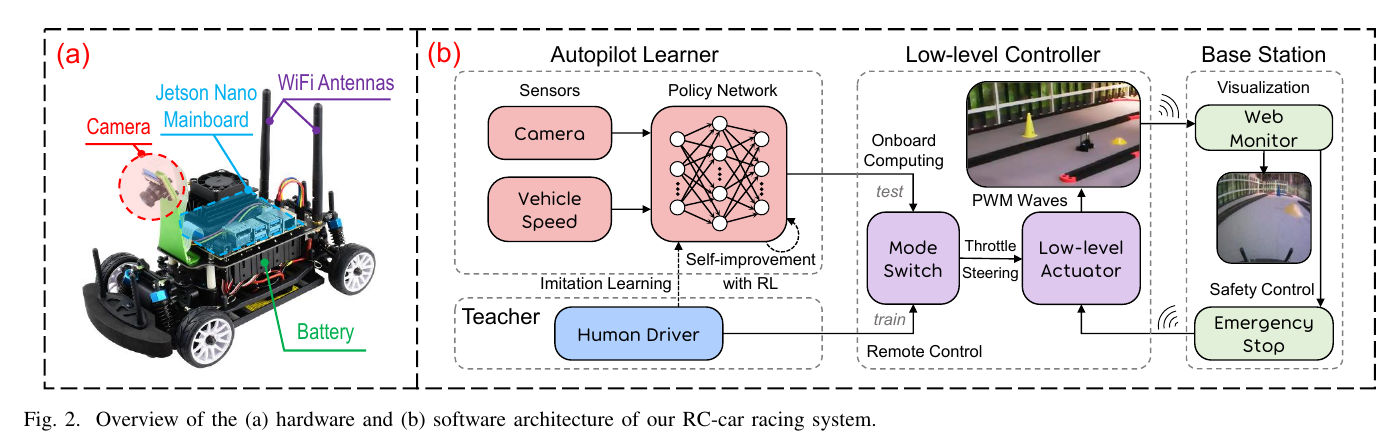
\includegraphics[width=\textwidth]{img/21}\label{fig:21}
    \end{subfigure}
    \begin{subfigure}{0.4\textwidth}
        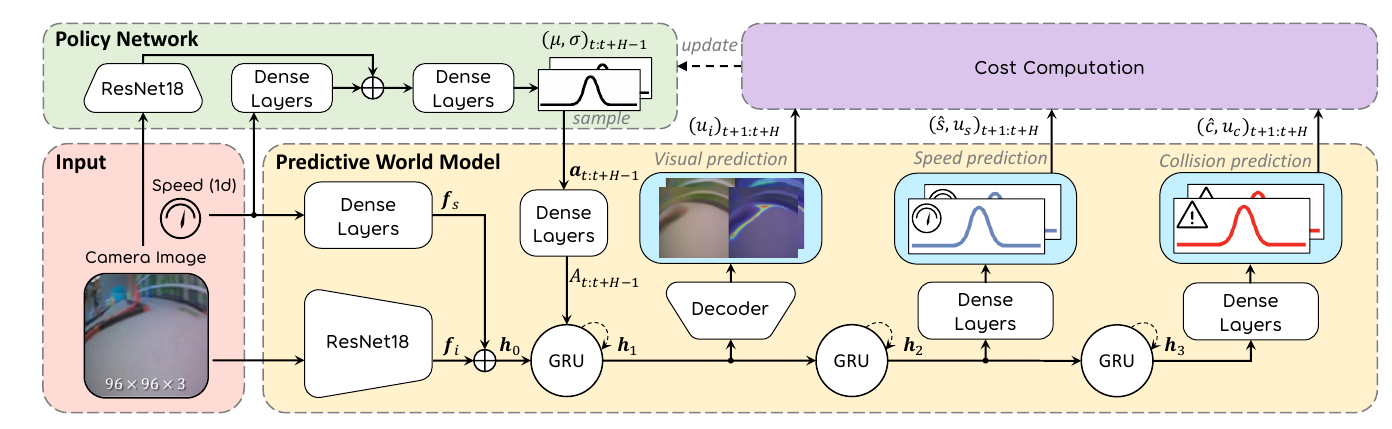
\includegraphics[width=\textwidth]{img/22}\label{fig:22}
    \end{subfigure}
%            \begin{subfigure}
%                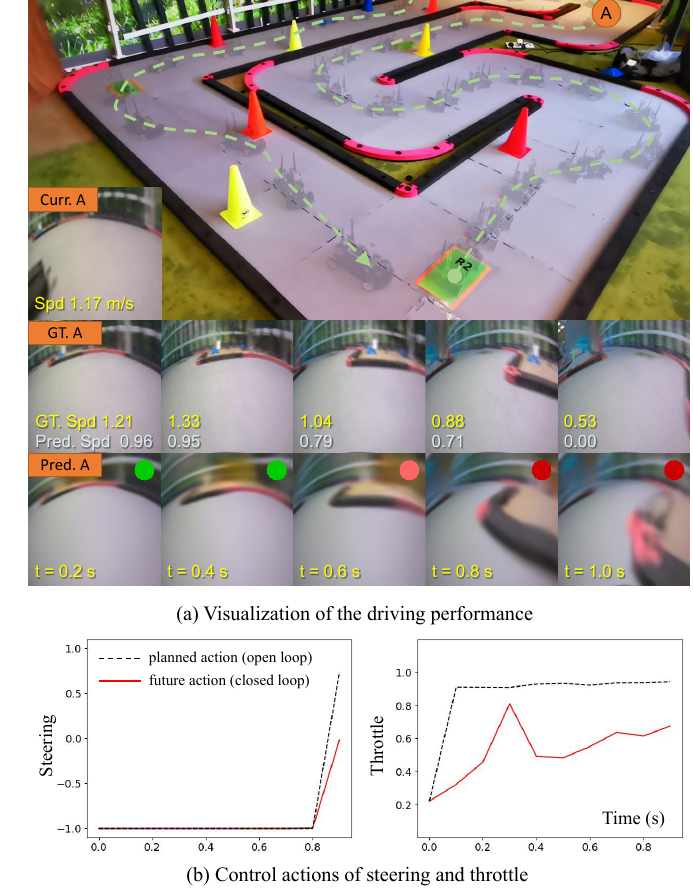
\includegraphics[width=0.2\textwidth]{img/23}\label{fig:23}
%            \end{subfigure}
\end{figure}

\clearpage

\noindent\textbf{Model-based probabilistic collision detection in autonomous driving}~\cite{althoff2009model}
El artículo fue publicado en la revista IEEE Transactions on Intelligent Transportation Systems en 2009 y se centra en la seguridad vial
de los vehículos autónomos en entornos de tráfico complejo.
Su enfoque principal es la detección probabilística de colisiones mediante el análisis y la predicción de la ocupación de la carretera
por parte de otros vehículos.\\
El estudio aborda la incertidumbre inherente en la interacción entre los vehículos autónomos y otros actores del tráfico.
Analiza cómo las mediciones y los posibles comportamientos de estos afectan la predicción de posibles colisiones.
Además, considera las limitaciones en las maniobras de conducción debidas a la geometría de la carretera y la influencia
de estas restricciones en la probabilidad de colisión para trayectorias específicas.\\
Lo más destacado de este enfoque es su eficiencia. La mayor parte de los cálculos intensivos se llevan a cabo offline,
permitiendo disponer de un algoritmo en línea eficiente para aplicaciones en tiempo real.                                                                           \\
Esto contribuye significativamente a la seguridad vial al proporcionar una herramienta precisa y eficaz para la detección anticipada de
posibles colisiones en entornos de conducción autónoma.                                                            \\
\begin{figure}[!ht]
    \begin{subfigure}{0.4\textwidth}
        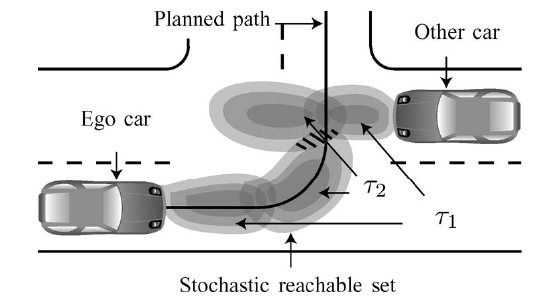
\includegraphics[width=\textwidth]{img/31}\label{fig:31}
    \end{subfigure}
    \begin{subfigure}{0.4\textwidth}
        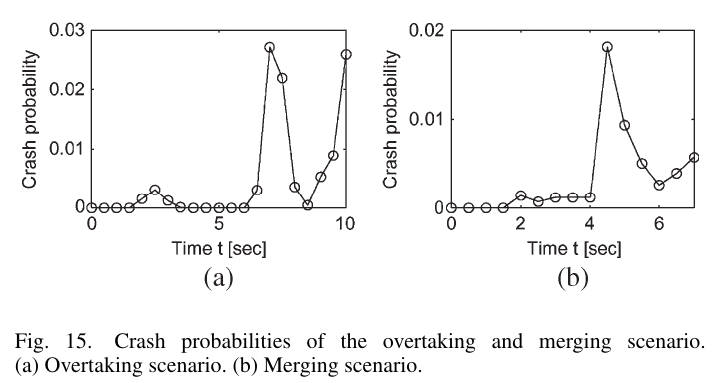
\includegraphics[width=\textwidth]{img/35}\label{fig:35}
    \end{subfigure}
%            \begin{subfigure}
%                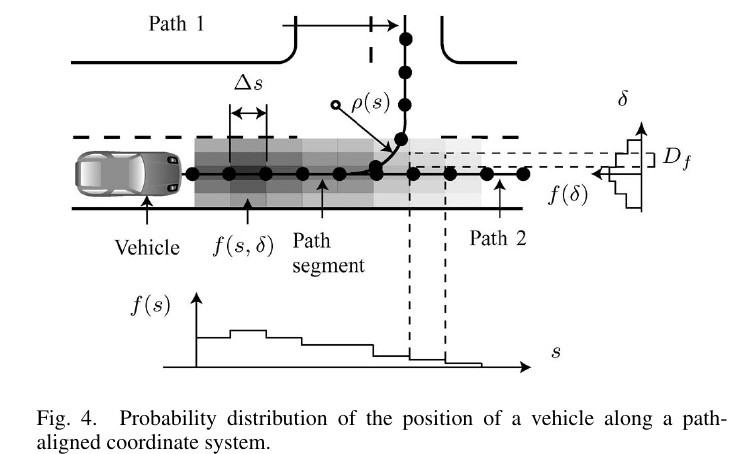
\includegraphics[width=0.5\textwidth]{img/32}\label{fig:32}
%            \end{subfigure}
    \vspace{2cm}
    \begin{subfigure}{0.4\textwidth}
        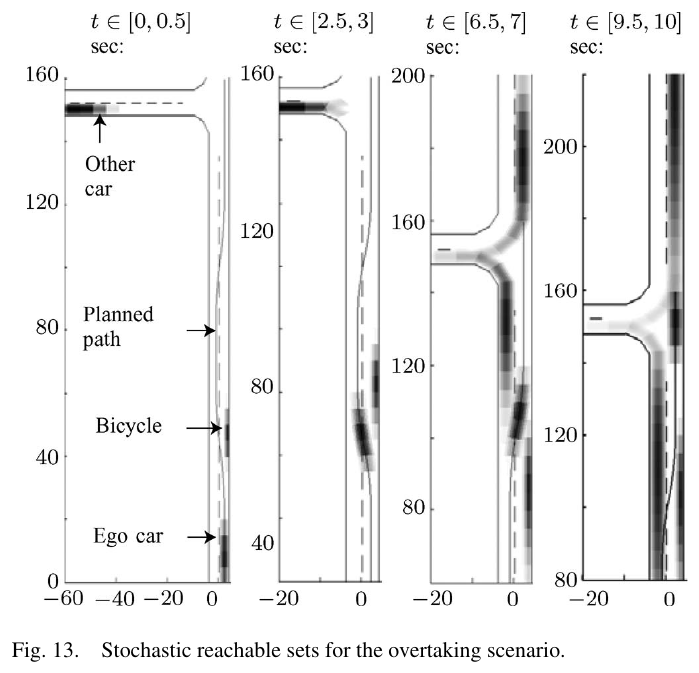
\includegraphics[width=\textwidth]{img/33}\label{fig:33}
    \end{subfigure}
    \begin{subfigure}{0.4\textwidth}
        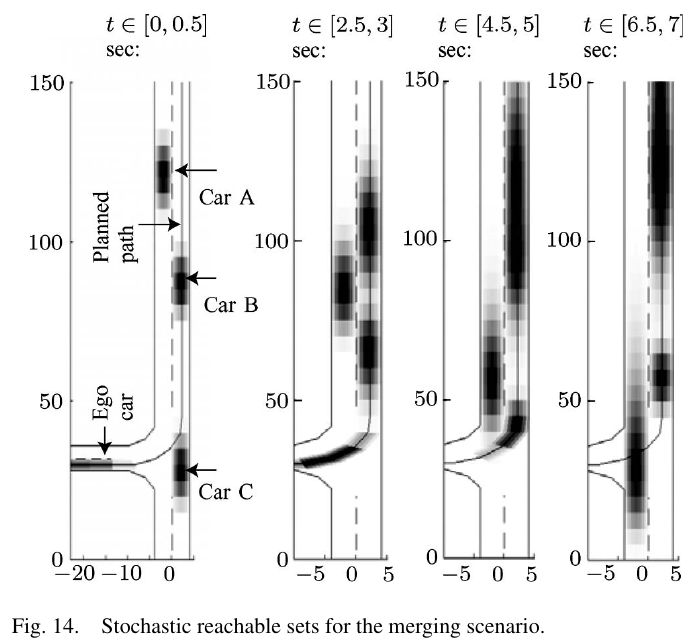
\includegraphics[width=\textwidth]{img/34}\label{fig:34}
    \end{subfigure}

\end{figure}
\clearpage

\noindent\textbf{Vision-based autonomous vehicle systems based on deep learning: A systematic literature review}~\cite{pavel2022vision}
El artículo fue publicado en la revista Applied Science en 2022 y presenta una revisión sistemática de la literatura sobre el empleo
de técnicas de aprendizaje profundo en los sistemas
de vehículos autónomos a lo largo de la última década.                                                                    \\Esta revisión se divide en varios módulos que abarcan distintos aspectos,
desde el análisis de percepción y la toma de decisiones hasta el control, la planificación de trayectorias
y la visualización en sistemas de realidad aumentada tipo HUD.                                                                                                                   \\
Se examinan investigaciones llevadas a cabo entre 2011 y 2021 que se enfocan en la utilización de cámaras RGB como sensores principales
en estos sistemas. Se otorga especial atención a los resultados finales, destacando la visualización en sistemas de realidad aumentada
basados en HUD.                                                                                                      \\Esto incluye advertencias tempranas, marcadores en la carretera para mejorar la navegación y la seguridad, superposición
de información en vehículos y peatones en condiciones visuales extremas para reducir colisiones.
La revisión subraya los métodos actuales de aprendizaje profundo que se basan únicamente en la visión de cámaras RGB, prescindiendo de la
compleja fusión de sensores.                                                                     \\Se espera que este enfoque allane el camino para el desarrollo ágil de sistemas de vehículos autónomos,
siendo prácticos, eficientes y seguros en términos de costos.                                                               \\
\begin{figure}[!ht]
    \centering
    \begin{subfigure}{\textwidth}
        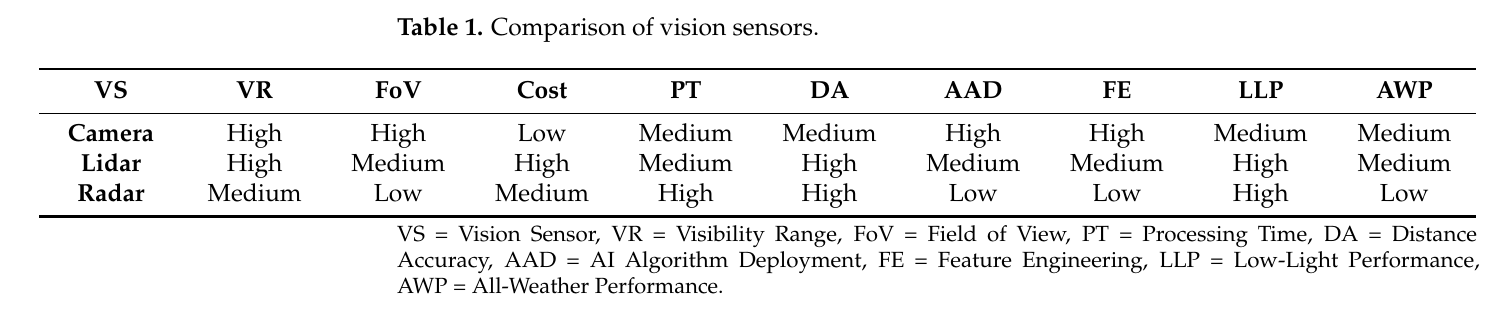
\includegraphics[width=1\textwidth]{img/71}\label{fig:71}
    \end{subfigure}
%            \begin{subfigure}
%                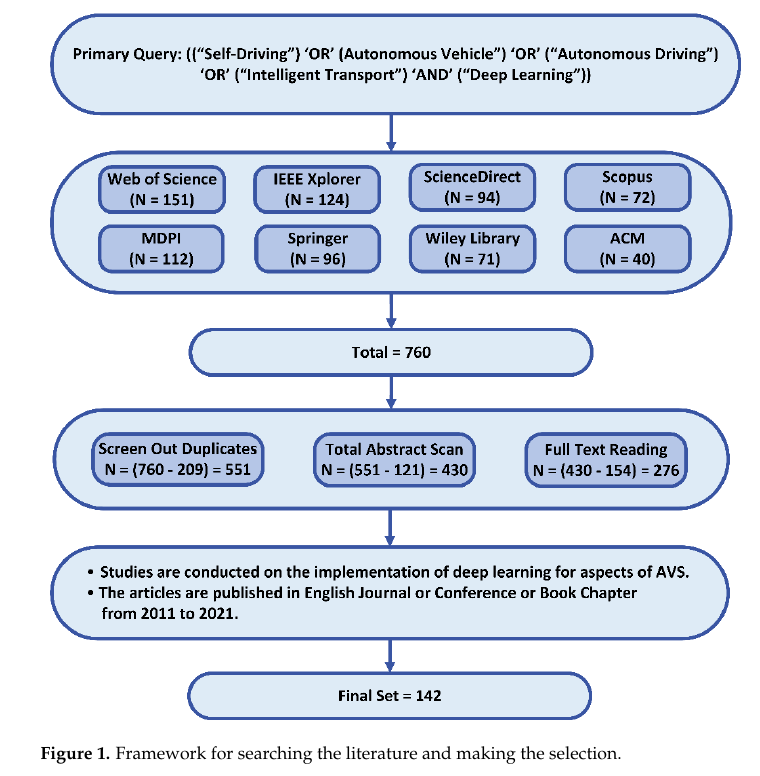
\includegraphics[width=0.5\textwidth]{img/72}\label{fig:72}
%            \end{subfigure}
    \begin{subfigure}{0.4\textwidth}
        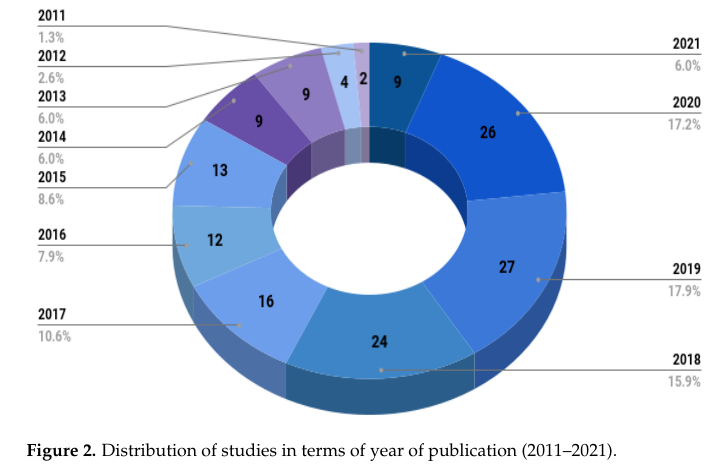
\includegraphics[width=\textwidth]{img/73}\label{fig:73}
    \end{subfigure}
    \begin{subfigure}{0.4\textwidth}
        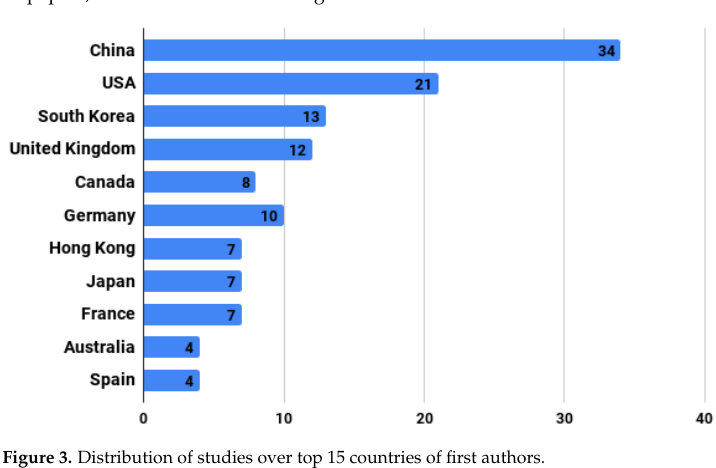
\includegraphics[width=\textwidth]{img/74}\label{fig:74}
    \end{subfigure}
\end{figure}
\clearpage

\noindent\textbf{A cost-effective computer vision-based vehicle detection system}~\cite{alam2022cost}
El artículo fue publicado en la revista Concurrent Engineering en 2022 y se enfoca en la detección de vehículos.
\\Destaca la importancia crítica del procesamiento rápido y la detección precisa de vehículos dentro de un sistema autónomo de detección.
\\Presenta un sistema de detección de vehículos basado en visión por computadora que utiliza un algoritmo de Gentle Adaptive Boosting
con características tipo Haar para generar hipótesis de vehículos de manera eficiente.
Para abordar los errores potenciales, propone el uso de un algoritmo de Máquinas de Vectores de Soporte (SVM) entrenado con características
del histograma de gradientes orientados (HOG) para filtrar las hipótesis falsas.
\\El descriptor HOG se centra en la forma y contornos de los vehículos, mejorando la precisión de la detección.
La combinación de características tipo Haar y HOG permite cumplir los objetivos de detección en la conducción autónoma.
\\El rendimiento del sistema propuesto se evalúa con imágenes capturadas durante el día y la noche y se compara con tres detectores
de vehículos existentes. Los resultados muestran una precisión promedio del 0.97 para imágenes capturadas durante el día
y del 0.94 para imágenes nocturnas.                                                                                               \\Además, se destaca que el sistema propuesto requiere aproximadamente 15 veces menos tiempo
de entrenamiento en comparación con las técnicas existentes, utilizando la misma cantidad de datos de imágenes y la misma unidad
de procesamiento central (CPU). Esto demuestra una mejora significativa en la eficiencia del sistema propuesto en términos de tiempo de entrenamiento.
\begin{figure}[!ht]
\centering
%            \begin{subfigure}
%                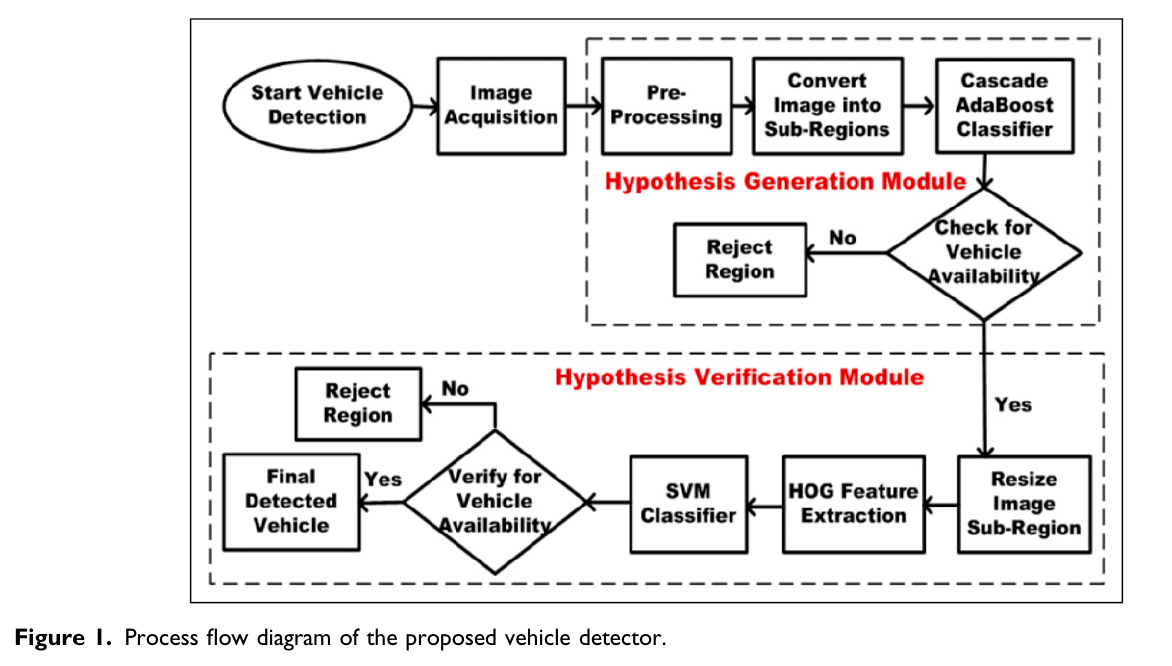
\includegraphics[width=0.6\textwidth]{img/81}\label{fig:81}
%            \end{subfigure}
%            \begin{subfigure}
%                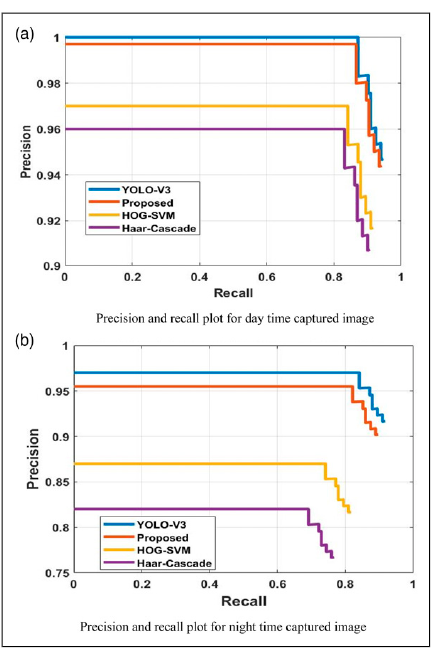
\includegraphics[width=0.5\textwidth]{img/86}\label{fig:82}
%            \end{subfigure}
    \begin{subfigure}{0.4\textwidth}
        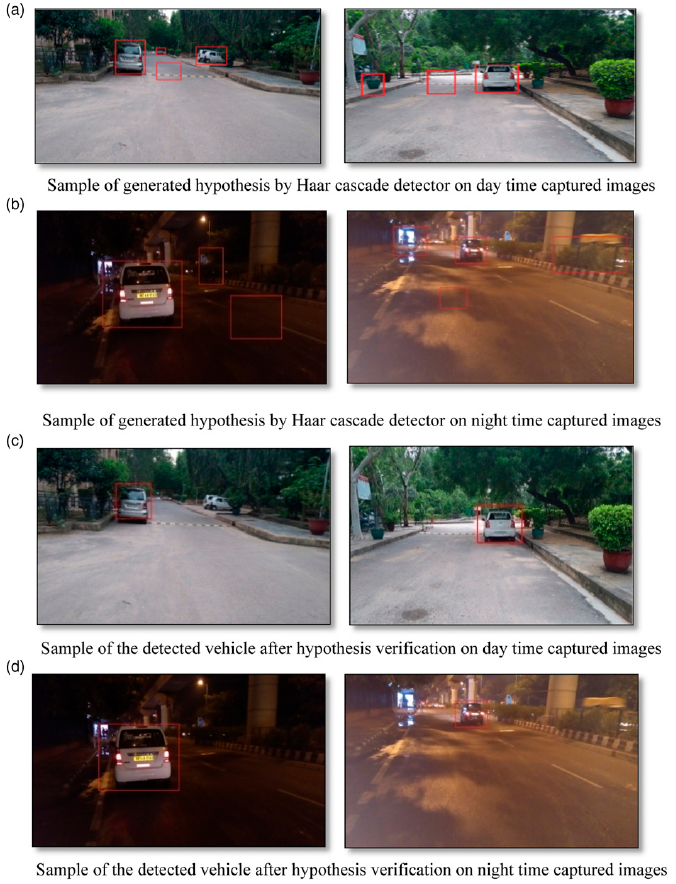
\includegraphics[width=\textwidth]{img/84}\label{fig:84}
    \end{subfigure}
    \begin{subfigure}{0.4\textwidth}
        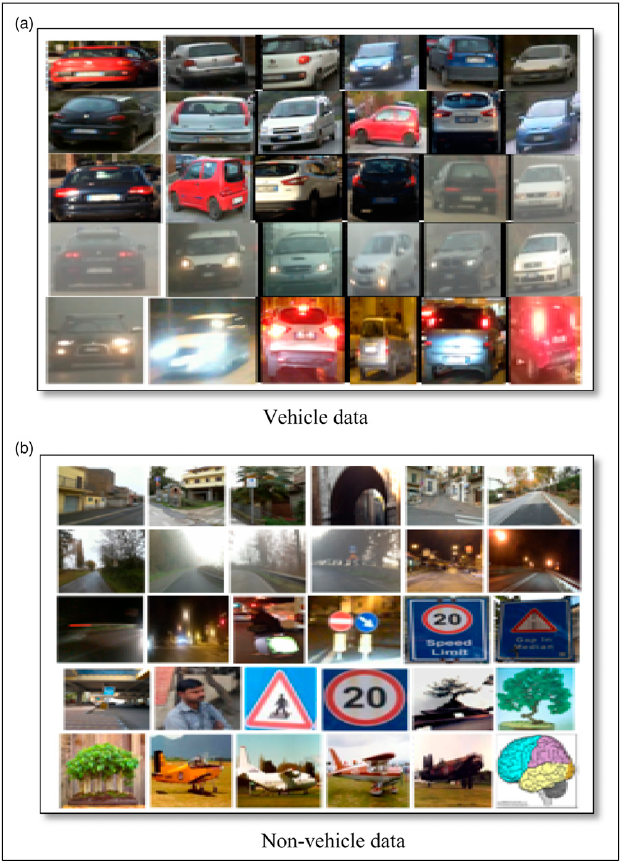
\includegraphics[width=\textwidth]{img/82}\label{fig:86}
    \end{subfigure}
\end{figure}
\clearpage


\subsubsection{Tabla comparativa}
\begin{center}
    \resizebox{\textwidth}{!}{
        \begin{tabular}{|p{5cm}|p{2cm}|p{2cm}|p{2cm}|p{2cm}|p{2cm}|p{2cm}|}
            \hline
            \textbf{Características}
            & \textbf{Propia}
            & \textbf{Autonomous Driving Architectures \cite{bachute2021autonomous}}
            & \textbf{Vision-based Autonomous Car Racing \cite{cai2021vision}}
            & \textbf{Model-based Probabilistic Collision Detection \cite{althoff2009model}}
            & \textbf{Vision-based Autonomous Vehicle Systems \cite{pavel2022vision}}
            & \textbf{Cost-effective Vehicle Detection System \cite{alam2022cost}} \\
            \hline
            Uso de algoritmos de Aprendizaje Automático y Aprendizaje Profundo & X & X &   &   & X &   \\
            \hline
            Enfoque en la conducción autónoma                                  & X & X & X & X & X & X \\
            \hline
            Ventajas de la conducción autónoma                                 & X & X &   &   &   &   \\
            \hline
            Complejidad de los sistemas de conducción autónoma                 &   & X &   &   &   &   \\
            \hline
            Análisis de tareas en la conducción autónoma                       & X & X &   &   &   &   \\
            \hline
            Evaluación y comparación de algoritmos                             &   & X & X &   &   &   \\
            \hline
            Predicción estocástica de ocupación de la carretera                &   &   &   & X &   &   \\
            \hline
            Eficiencia en cálculos intensivos                                  &   &   & X & X &   &   \\
            \hline
            Utilización de cámaras RGB como sensores principales               & X &   & X &   & X &   \\
            \hline
            Detección de vehículos en conducción autónoma                      & X &   &   &   &   & X \\
            \hline
        \end{tabular}
    }
\end{center}


% Capítulo 2: Metodología
\clearpage
\section{Metodología}
\noindent
La metodología propuesta se fundamenta en un enfoque iterativo que abarca diversas etapas para la implementación del sistema
de estimación de la posición relativa al estacionamiento de un vehículo mediante cámaras y sensores para estacionamiento automático en simulación.
En primera instancia, se establecerá un entorno de simulación realista que refleje el escenario de un vehículo en movimiento y su entorno de estacionamiento.
Posteriormente, se procederá a la adquisición y procesamiento de datos provenientes de los sensores de dicho entorno simulado.
La fase siguiente implicará el diseño y la implementación de algoritmos de visión computacional para la detección temprana de eventos críticos en tiempo real.
Estos algoritmos serán sometidos a un proceso de entrenamiento y ajuste utilizando técnicas de aprendizaje automático.
Finalmente, se llevarán a cabo pruebas exhaustivas y evaluaciones para validar la efectividad y la precisión del sistema propuesto en situaciones simuladas.

\subsection{Entorno de simulación}

%- Para resolver la problematica se propone una simulacion
%- una simulacion es
%- la simulacion nos puede ayudar en
%- podemos disenar la simulacion asi
%- los resultados obtenidos en la simulacion seran buen comienzo para lograr el objetivo en la vida real
\noindent
La simulación computacional se ha consolidado como una herramienta fundamental en el desarrollo y validación de sistemas de conducción autónoma.
Permite recrear escenarios complejos y peligrosos de manera segura, flexible y económica, facilitando la experimentación 
y el análisis de algoritmos antes de su implementación en vehículos reales. 
En el contexto de este trabajo, la simulación resulta especialmente útil para modelar situaciones de estacionamiento automático,
donde la precisión y la seguridad son críticas. 
A través de la simulación, es posible ajustar parámetros, evaluar el desempeño de sensores virtuales 
y analizar el comportamiento del sistema bajo diferentes condiciones ambientales y de tráfico, 
todo ello sin los riesgos y costos asociados a las pruebas físicas.
La simulación nos puede proporcionar información detallada del vehículo y su entorno en situaciones de estacionamiento,
lo que nos permitirá hacer mediciones y análisis detallados de los datos obtenidos similar a como se haría en la vida real.

\subsection{Carla Simulator}\label{subsec:carla-simulator}
\noindent
Para llevar a cabo la simulación propuesta, se utilizará: \texttt{%
    \href{https://github.com/carla-simulator/carla}{%
        CARLA Simulator}%
}
, (Car Learning to Act)una plataforma de código abierto ampliamente utilizada en la investigación de vehículos autónomos~\cite{dosovitskiy2017carla}.
 CARLA destaca por su capacidad de generar entornos urbanos realistas, con una amplia variedad de modelos de vehículos, peatones, señales de tráfico
  y condiciones ambientales configurables, como clima y hora del día. 
  Además, permite la integración de múltiples sensores virtuales (cámaras, LIDAR, radar, GPS, entre otros),
   lo que facilita la obtención de datos similares a los que se recopilarían en un vehículo real. 
   Esta flexibilidad convierte a CARLA en una herramienta idónea para el desarrollo, prueba y validación de algoritmos de percepción, 
   localización y control en escenarios de estacionamiento automático, permitiendo iterar rápidamente sobre diferentes configuraciones 
   y estrategias sin comprometer la seguridad.
\noindent
Varias de estas condiciones ambientales se ilustran en la figura~\ref{fig:carla-simulator}.

\begin{figure}[!ht]
    \centering
    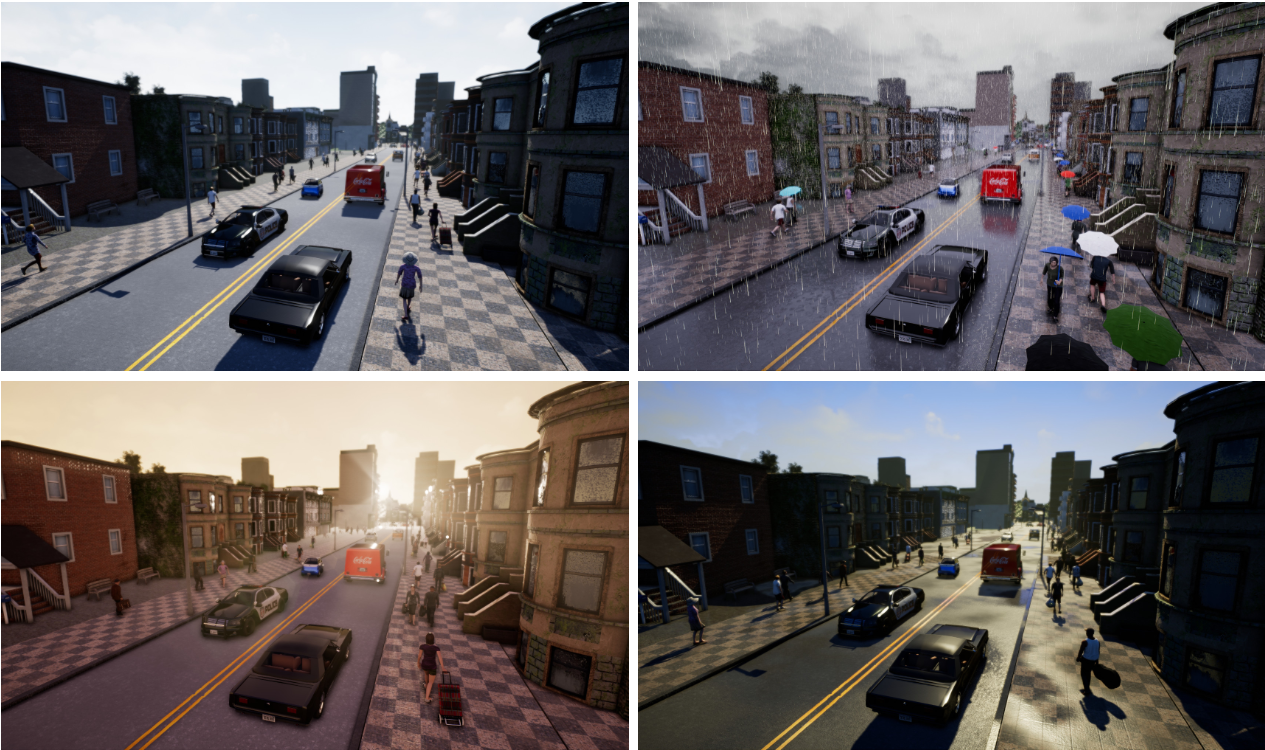
\includegraphics[width=0.8\textwidth]{img/carla_clima_example}
    \caption{Condiciones ambientales en el simulador CARLA.}
    \label{fig:carla-simulator}
\end{figure}


\subsection{Diseño del entorno de simulación}\label{subsec:simulation-design}
\noindent
Para modelar el entorno de simulación, se propone un escenario de estacionamiento que incluye un vehículo y un espacio de estacionamiento.
La ubicación del vehículo se inicializará de manera aleatoria en este espacio.
El vehículo estará equipado con sensores que proporcionarán los datos de entrada que se utilizarán para estimar la posición del vehículo con respecto al espacio de estacionamiento.
Estos sensores incluirán cámara y velocímetro para capturar de manera similar a como se haría en la vida real.
En la figura~\ref{fig:simulation-design} se muestra un ejemplo de cómo se podría diseñar el entorno de simulación.

\begin{figure}[!ht]
    \centering
    \begin{subfigure}{0.4\textwidth}
        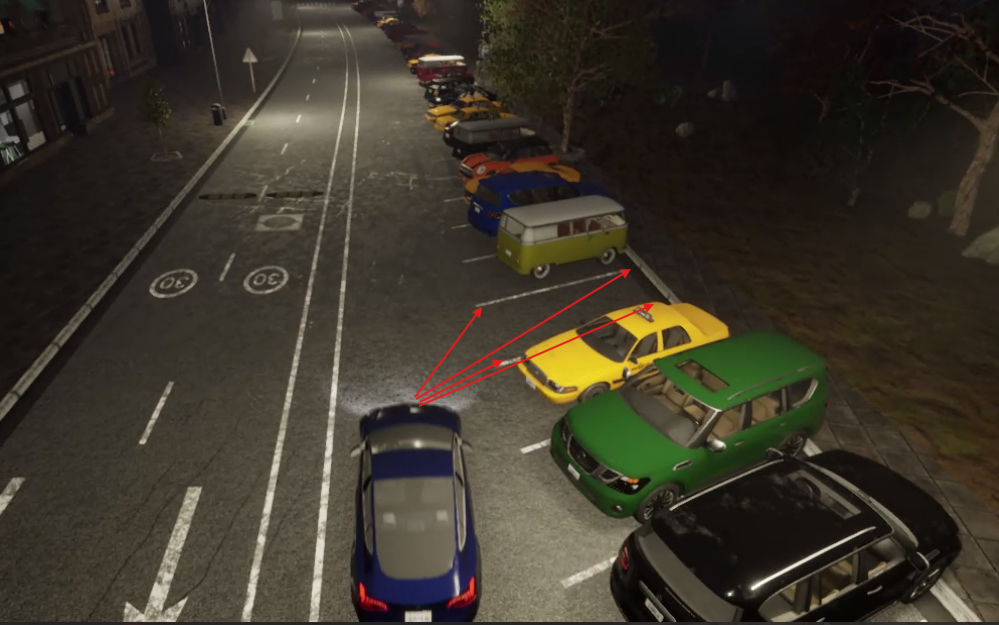
\includegraphics[width=\textwidth]{img/distances}\label {fig:distances}
    \end{subfigure}
    \begin{subfigure}{0.4\textwidth}
        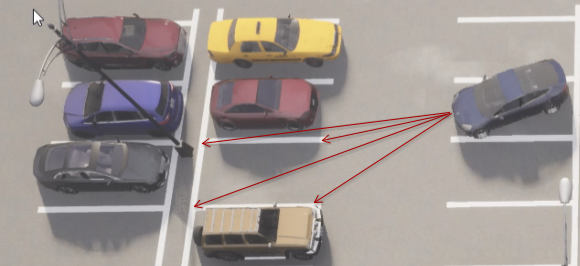
\includegraphics[width=\textwidth]{img/distances2}\label {fig:distances2}
    \end{subfigure}
    
    \caption{Diseño del entorno de simulación en CARLA.}
    \label{fig:simulation-design}
\end{figure}

\noindent
La cámara del vehículo capturará imágenes del entorno y el espacio de estacionamiento y el simulador permite ubicarla a conveniencia en el vehículo.
La ubicación de la cámara estará en la zona delantera del vehículo a una altura conocida (detrás del retrovisor).
La figura ~\ref{fig:camera-view} muestra un ejemplo de como se visualiza el entorno desde la perspectiva de la cámara.

\begin{figure}[!ht]
    \centering
    \begin{subfigure}{0.4\textwidth}
        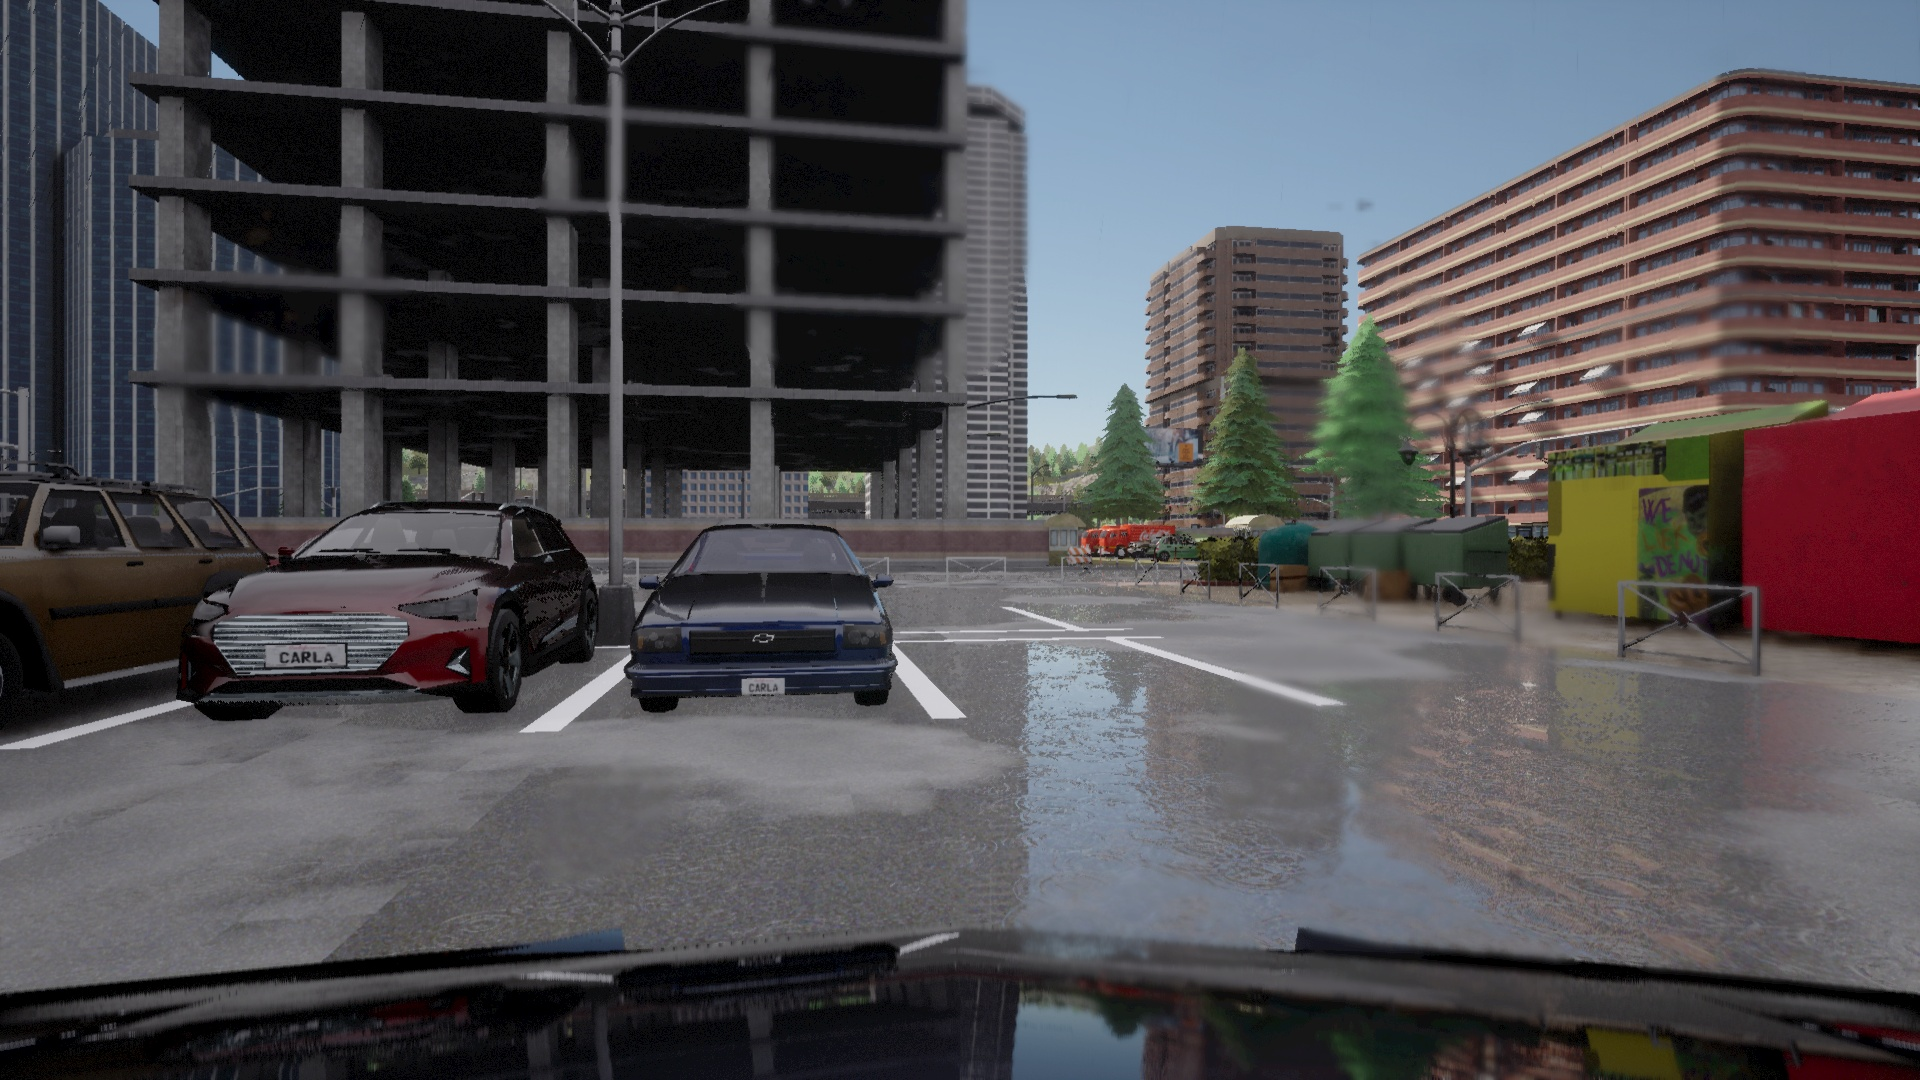
\includegraphics[width=\textwidth]{img/mirrow_camara_ex}\label {fig:camara}
    \end{subfigure}
    \begin{subfigure}{0.4\textwidth}
        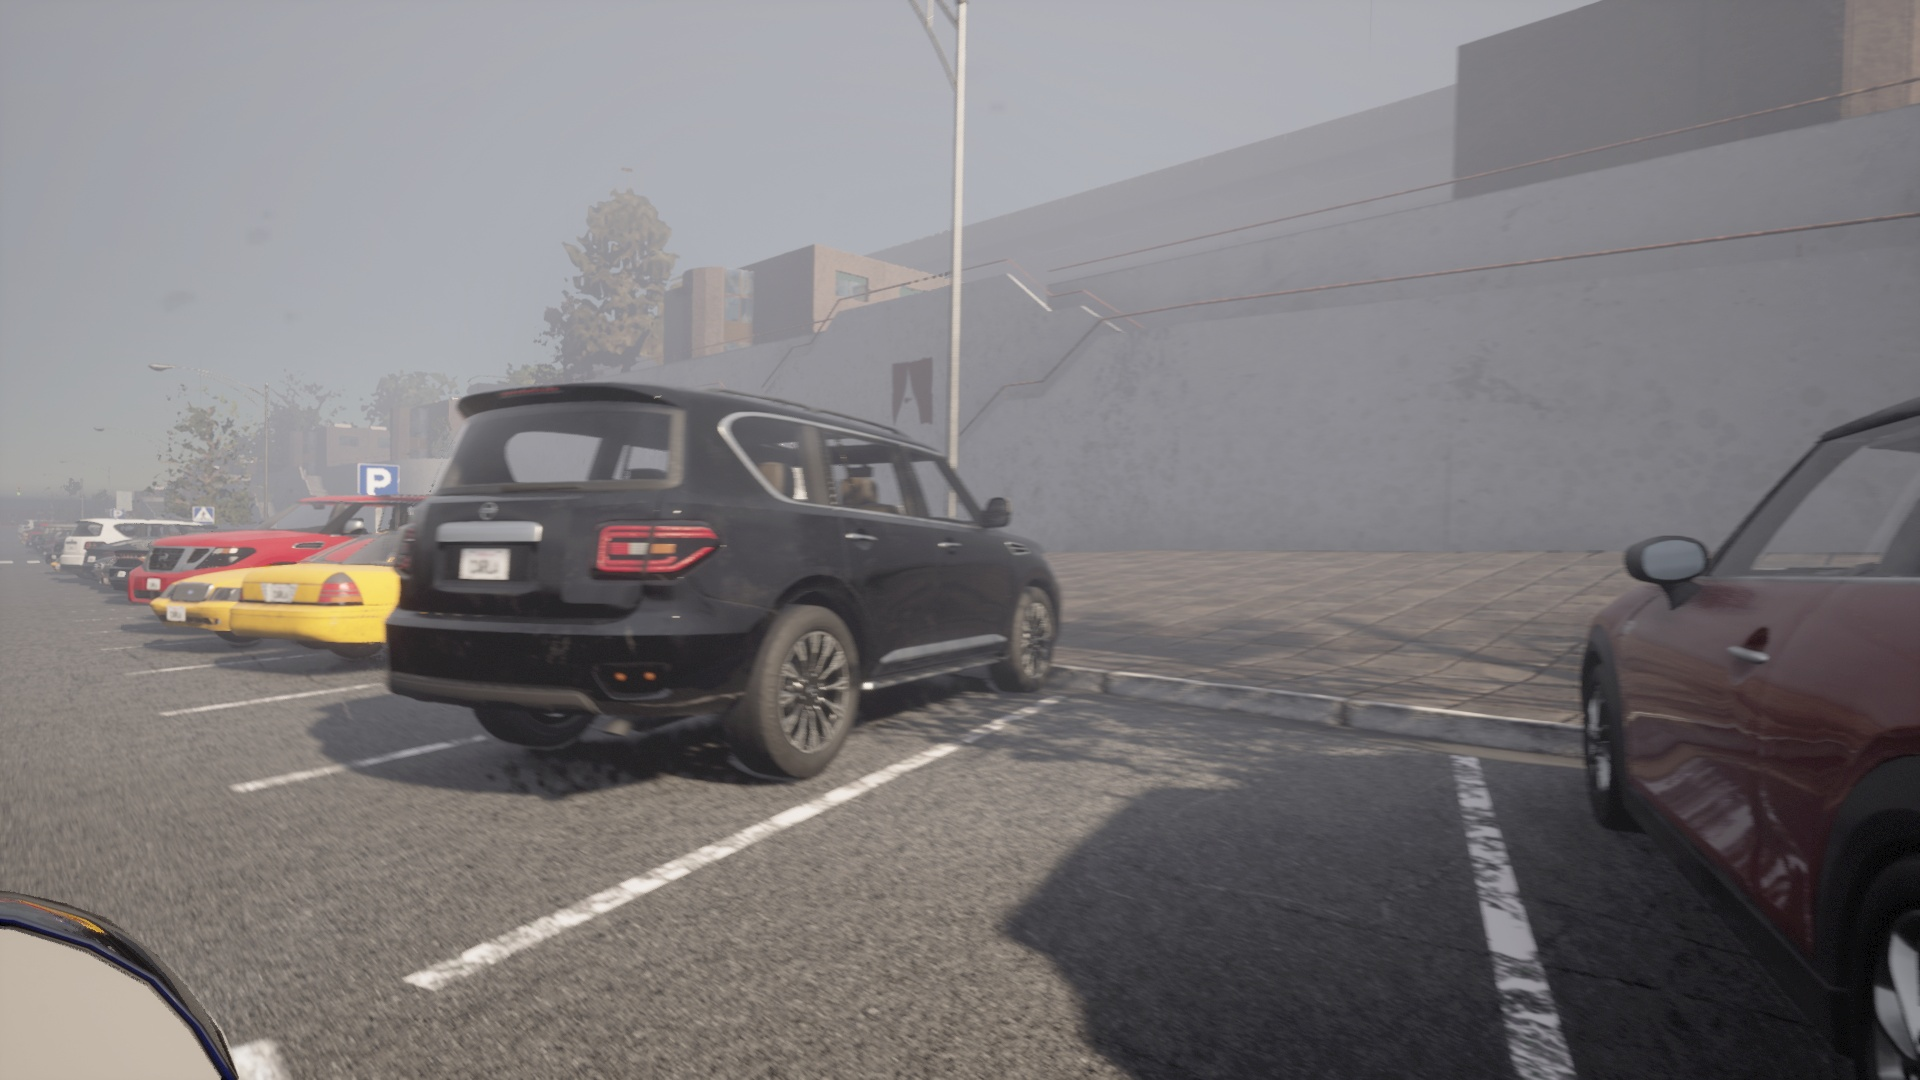
\includegraphics[width=\textwidth]{img/mirrow_camara_ex2}\label {fig:camara2}
    \end{subfigure}
    \caption{Vista de la cámara en el entorno de simulación.}
    \label{fig:camera-view}
\end{figure}






\subsection{Detección de la retícula de estacionamiento}
\noindent
Cuando proyectamos una escena del mundo real en tres dimensiones sobre un plano bidimensional, como la película o el sensor de una cámara, se produce una transformación en la imagen.
Esta transformación, conocida como transformación proyectiva, provoca que las líneas paralelas en el mundo real, al proyectarse en el plano de la cámara, se intersecten en un punto denominado punto de fuga.

\begin{figure}[!ht]
    \centering
    \begin{subfigure}{0.4\textwidth}
        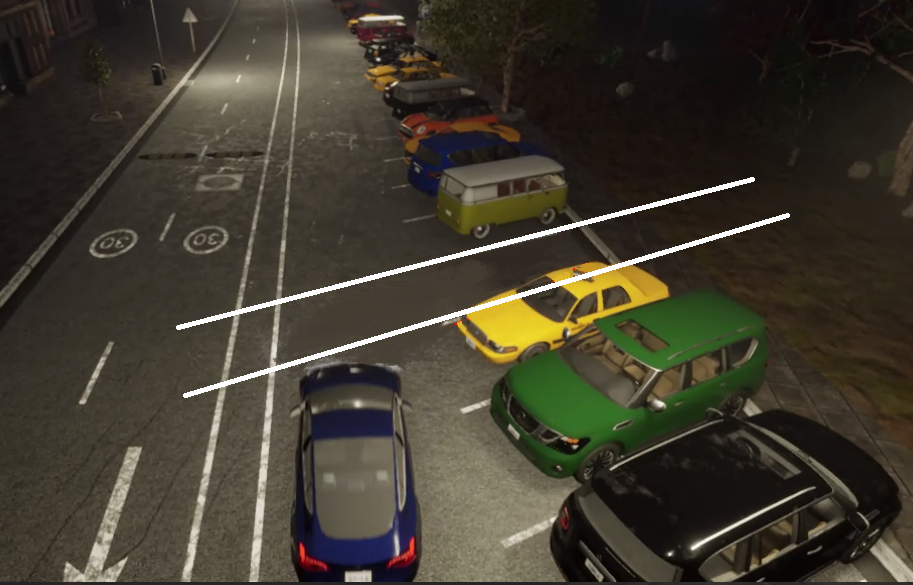
\includegraphics[width=\textwidth]{img/reticule/paralel_lines}\label{fig:parallel_lines}
        \caption{Ejemplo de líneas paralelas en un escenario real en tres dimensiones.}
    \end{subfigure}
    \begin{subfigure}{0.4\textwidth}
        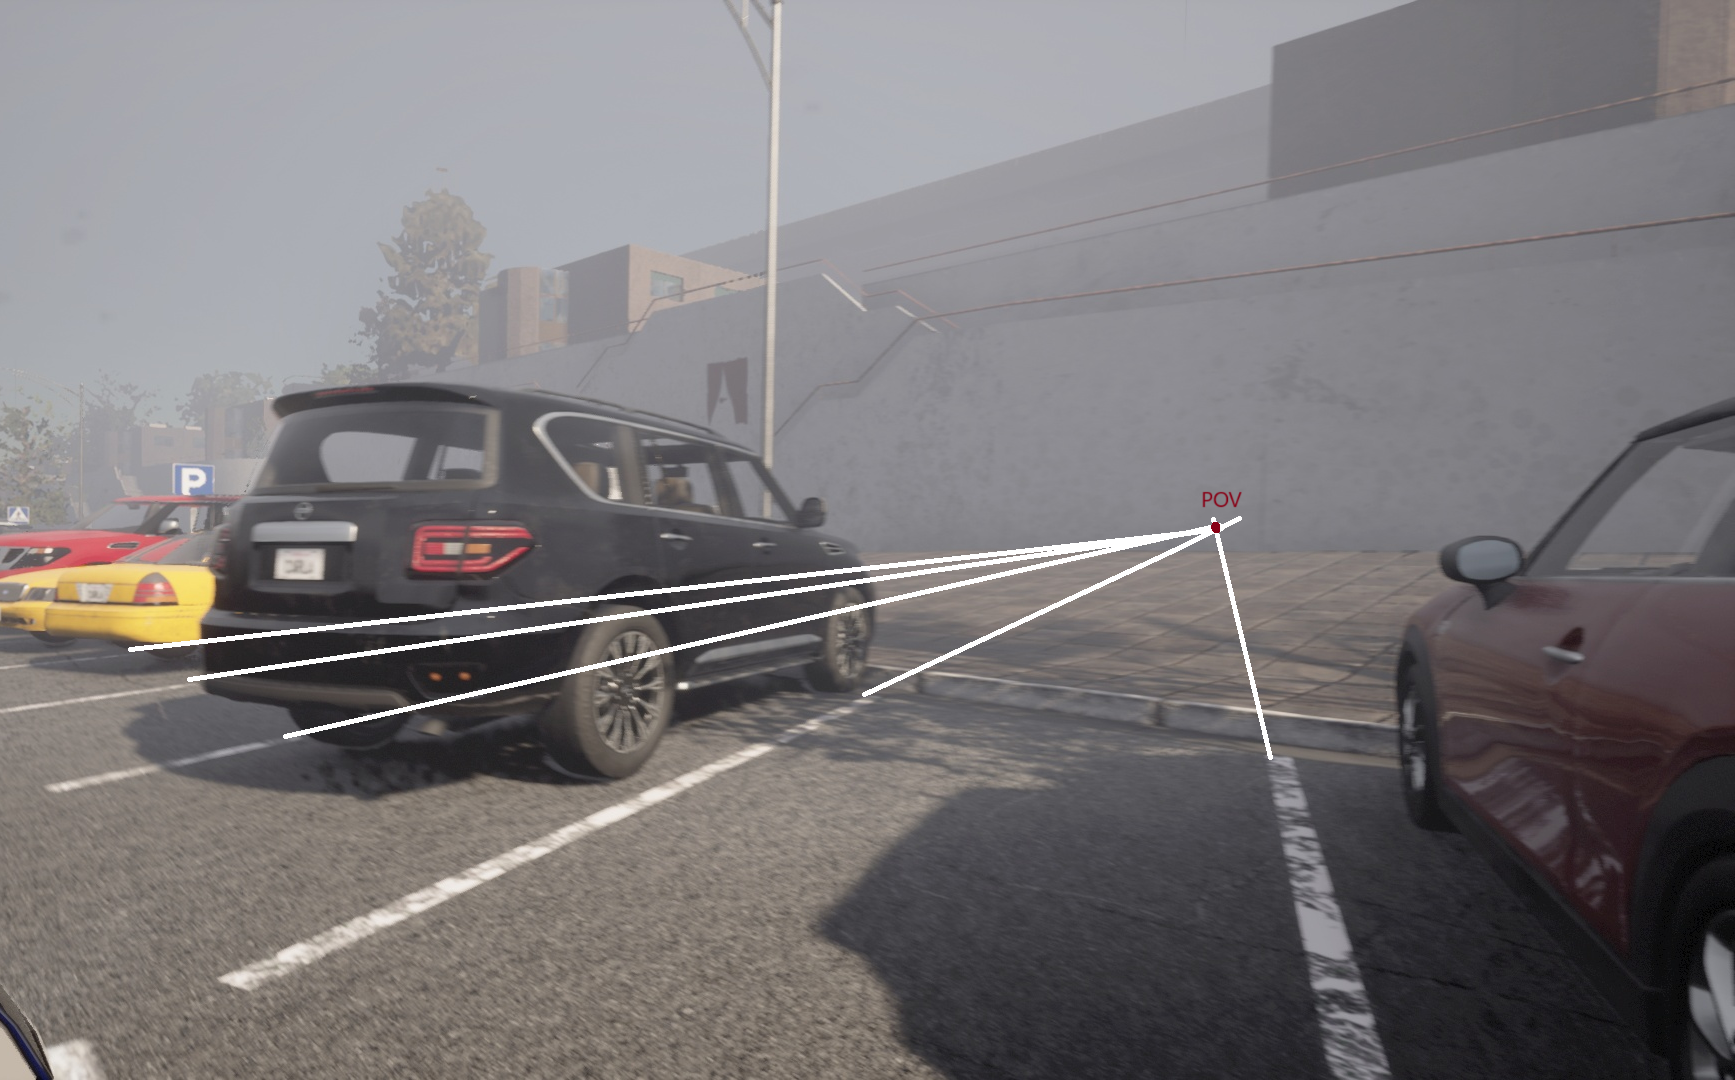
\includegraphics[width=\textwidth]{img/reticule/pov}\label{fig:pov}
        \caption{Proyección de líneas paralelas en el plano de la cámara.}
    \end{subfigure}

    \label{fig:distorion}
\end{figure}

\noindent
Dado que las líneas de los cajones de estacionamiento son paralelas por su geometría, forman patrones en una retícula de paralelogramos.
Esto permite utilizar técnicas de detección de líneas para identificar los puntos de fuga y estimar la posición de la retícula de estacionamiento.
En la figura \ref{fig:reticule_pov} se muestra un ejemplo de la retícula de estacionamiento vista desde la perspectiva de la cámara del vehículo.

\begin{figure}[!ht]
    \centering
    \begin{subfigure}{0.8\textwidth}
        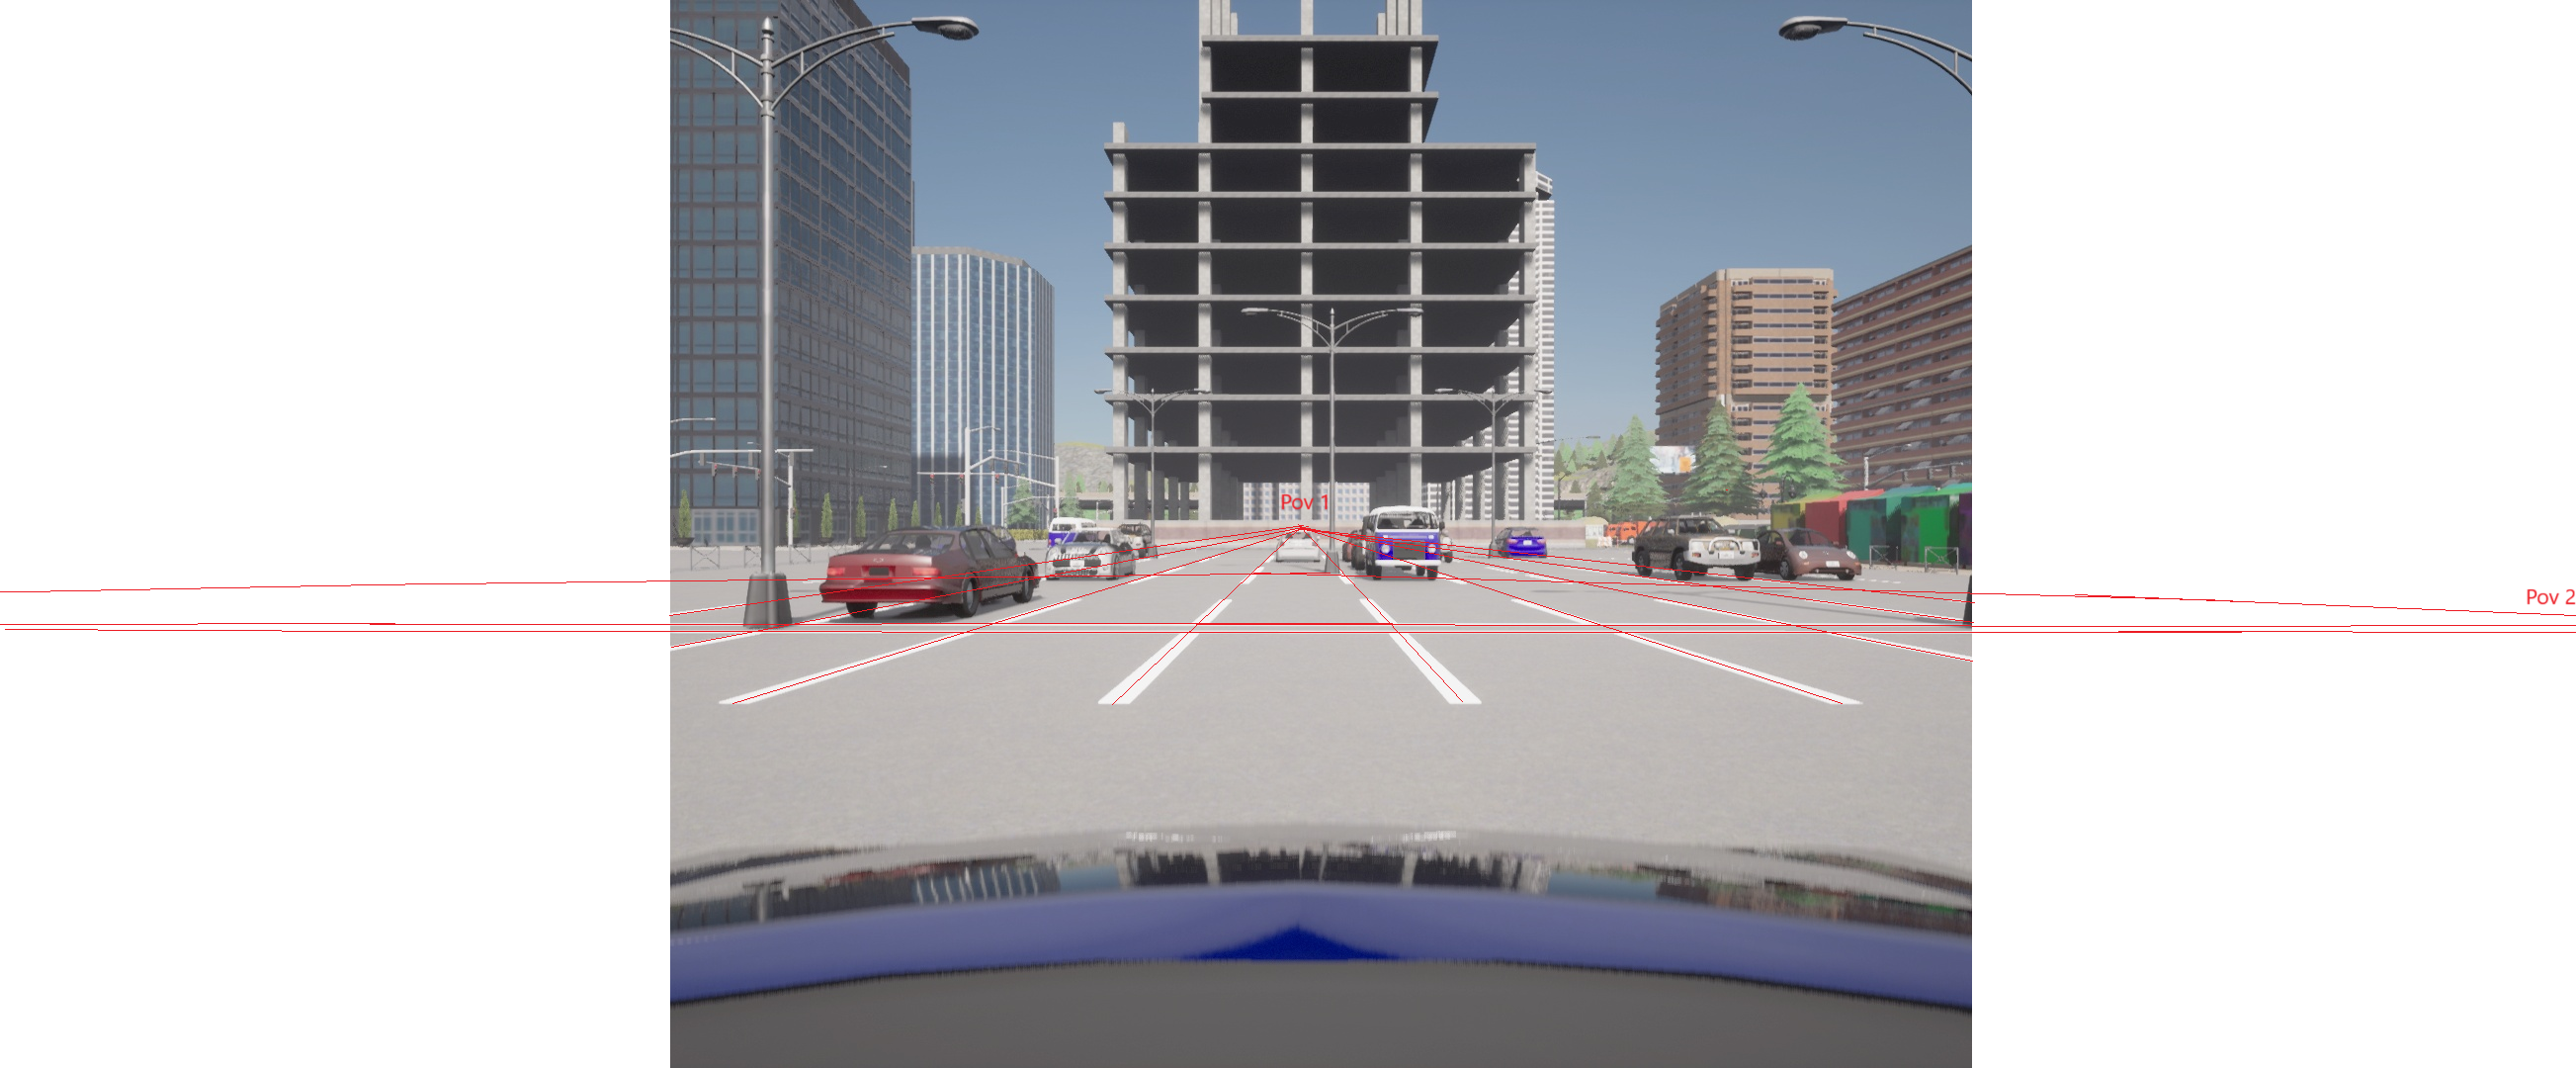
\includegraphics[width=\textwidth]{img/reticule/pov_reticule}\label{fig:pov_reticule}
    \end{subfigure}
    \begin{subfigure}{0.8\textwidth}
        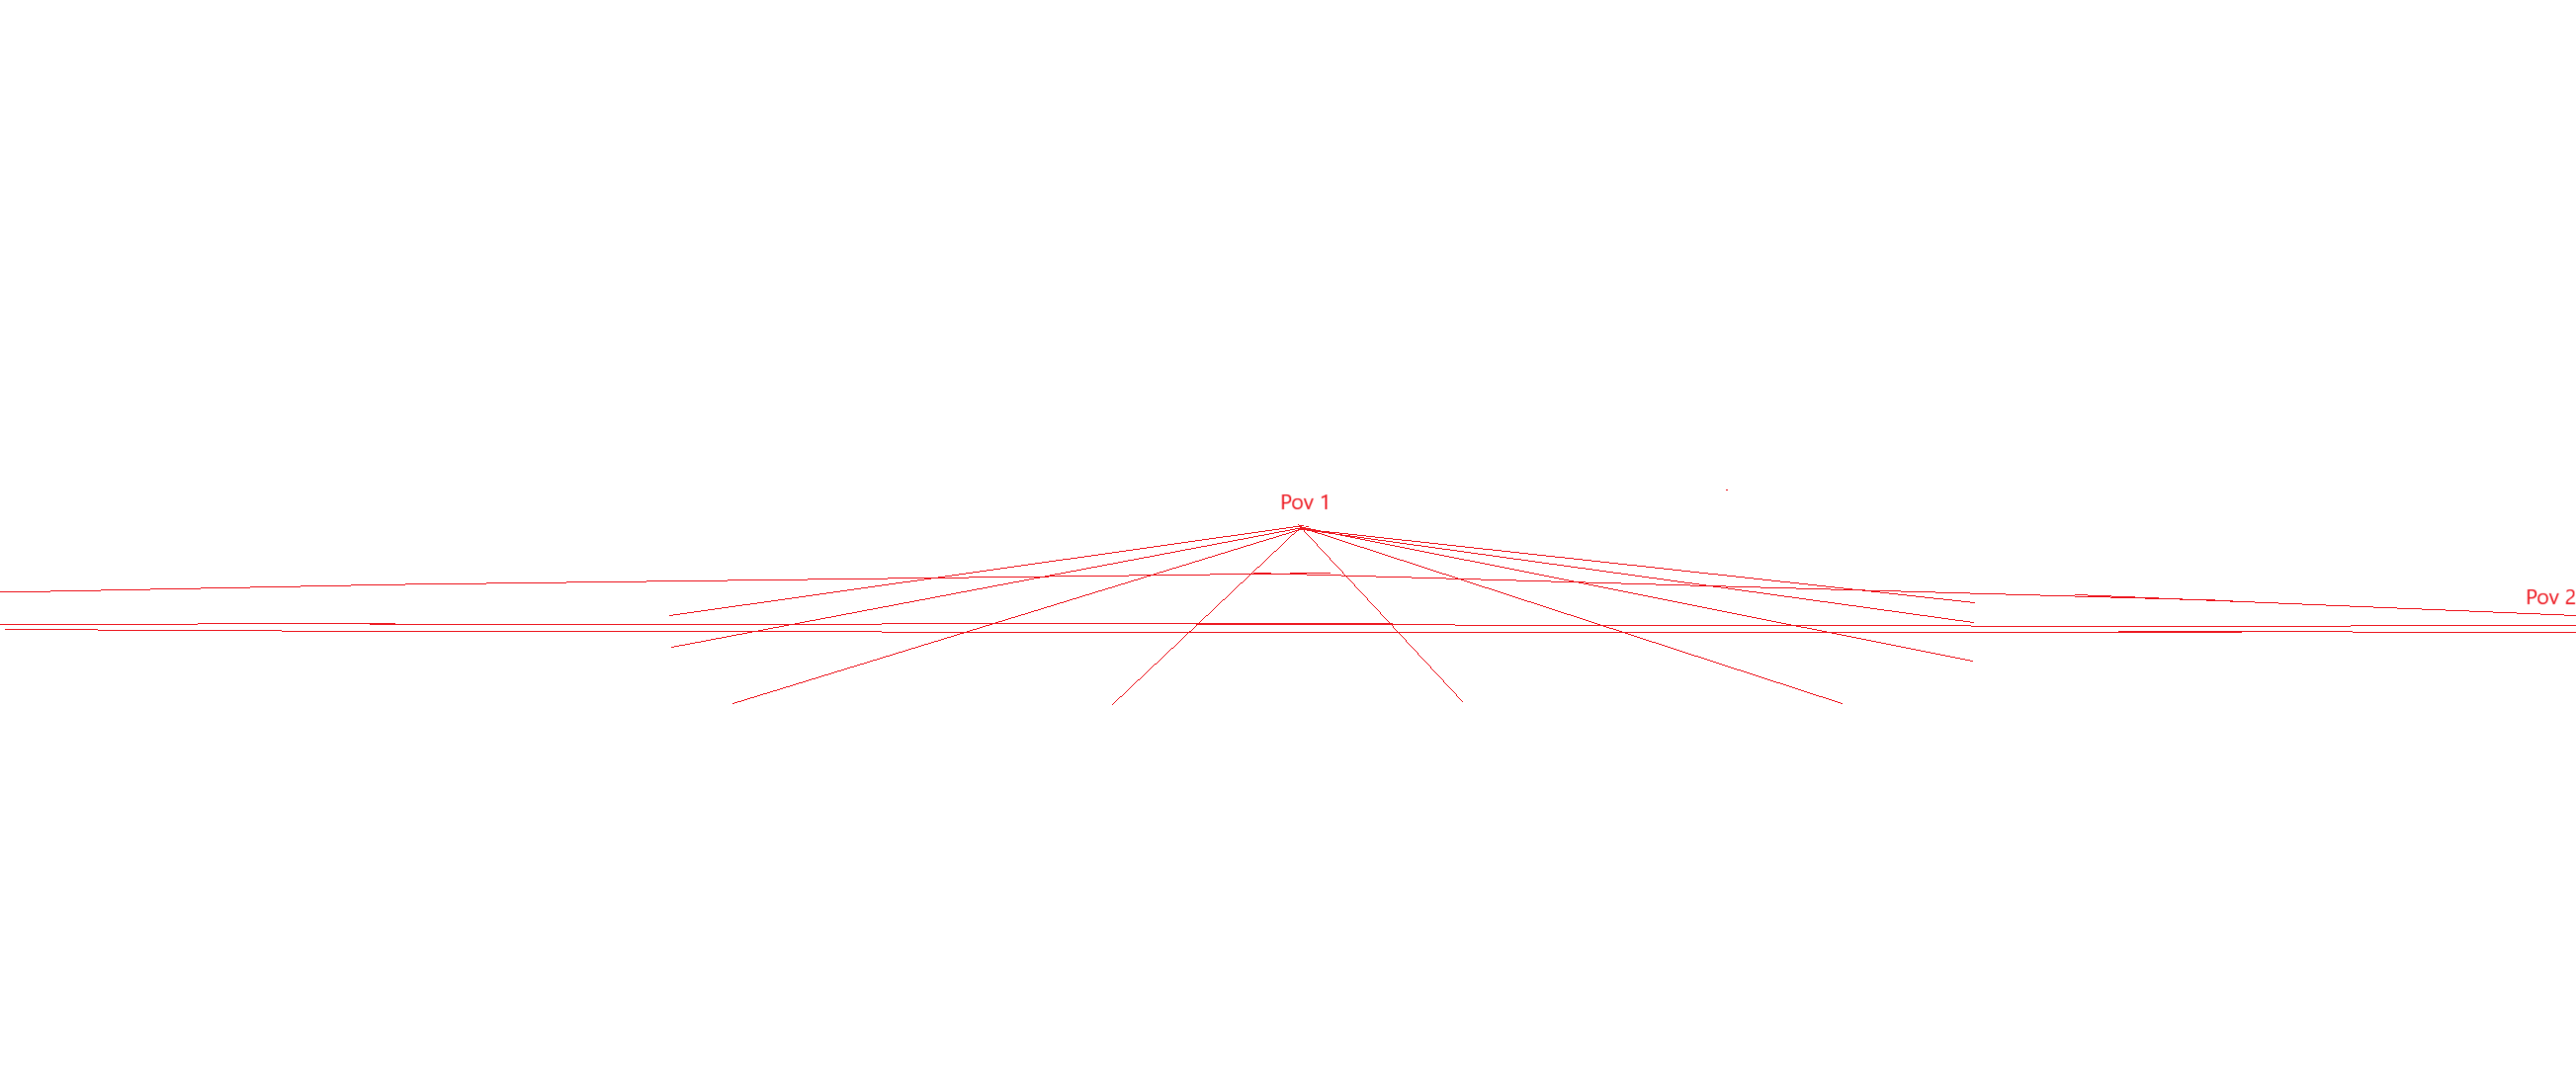
\includegraphics[width=\textwidth]{img/reticule/pov_reticule_layer}\label{fig:pov_reticule_layers}
    \end{subfigure}
    \caption{Líneas paralelas de la retícula de estacionamiento.}
    \label{fig:reticule_pov}
\end{figure}

\noindent
En esta sección se describen los pasos prácticos para identificar y analizar las líneas paralelas presentes en la imagen,
esenciales para la estimación de la retícula de estacionamiento.
El enfoque se centra en el procesamiento de la imagen y la extracción de información geométrica relevante,
utilizando técnicas clásicas de visión computacional.


\subsubsection{Área de interés:}
\noindent
Teniendo en cuenta que la cámara del vehículo se encuentra ubicada en la parte delantera a una altura conocida y en un ángulo paralelo al suelo, el área de interés de la imagen donde se encuentran las líneas de los cajones de estacionamiento quedará siempre por debajo del horizonte de la imagen.
Por lo tanto, se puede eliminar la parte superior de la imagen para
reducir el ruido y mejorar la detección de las líneas, como se muestra en la figura \ref{fig:roi}. \\
\begin{figure}[!ht]
    \centering
    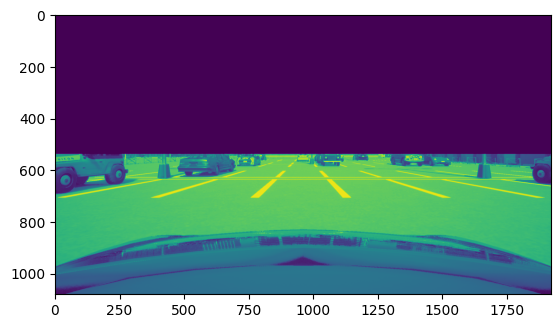
\includegraphics[width=0.8\textwidth]{img/reticule/horizont}
    \caption{Área de interés de la imagen}
    \label{fig:roi}
\end{figure}

\subsubsection{Umbralización:}
\noindent
Al área de interés de la imagen se le aplica una umbralización para realzar las líneas blancas de los cajones de estacionamiento
y eliminar otros elementos no relevantes que puedan interferir en la detección.
En la figura \ref{fig:threshold} se muestra un ejemplo de la imagen umbralizada.
\begin{figure}[!ht]
    \centering
    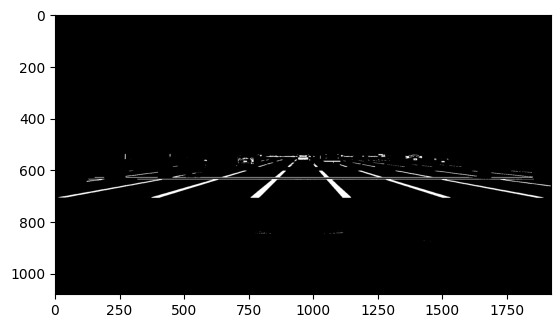
\includegraphics[width=0.8\textwidth]{img/reticule/thresholded}
    \caption{Imagen umbralizada}
    \label{fig:threshold}
\end{figure}

\subsubsection{Detección de contornos (Canny):}
\noindent
Se utiliza el algoritmo de Canny \cite{canny1986edge} para detectar los bordes de las líneas en la imagen umbralizada.
En la figura \ref{fig:edges} se muestra un ejemplo de la imagen con los bordes detectados.
\begin{figure}[!ht]
    \centering
    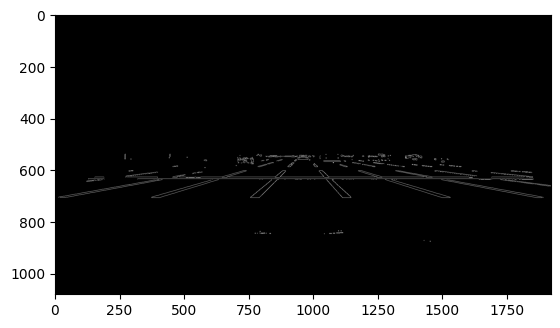
\includegraphics[width=0.6  \textwidth]{img/reticule/canny}
    \caption{Detección de bordes mediante el algoritmo de Canny}
    \label{fig:edges}
\end{figure}

\subsubsection{Detección de líneas (Hough):}
\noindent
Se aplica la transformada de Hough \cite{ballard1981hough} para detectar las coordenadas de inicio y fin de las líneas en la imagen.
En las figuras \ref{fig:hough} y \ref{fig:lines} se muestran las líneas detectadas sin fondo y sobre la imagen original, respectivamente.
\begin{figure}[!ht]
    \begin{subfigure}{0.5\textwidth}
        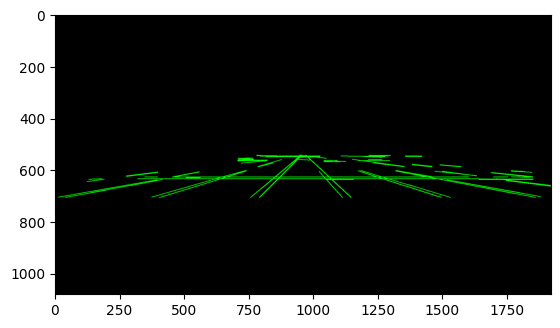
\includegraphics[width=\textwidth]{img/reticule/hough2}
        \caption{Líneas detectadas con la transformada de Hough}
        \label{fig:hough}
    \end{subfigure}
    \begin{subfigure}{0.5\textwidth}
        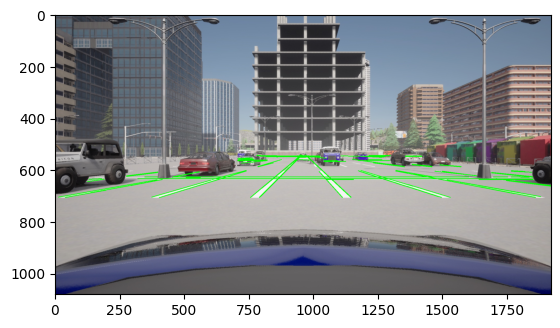
\includegraphics[width=\textwidth]{img/reticule/hough}
        \caption{Líneas detectadas en la imagen original}
        \label{fig:lines}
    \end{subfigure}
\end{figure}

\subsubsection{Representación de las ecuaciones de las líneas:}
\noindent
Una vez obtenidas las coordenadas de inicio y fin de cada línea paralela, se puede utilizar la ecuación general de la recta:
\begin{equation}
    Ax + By + C = 0
\end{equation}
Esta ecuación permite determinar la orientación de cada línea.
Dado que las coordenadas iniciales y finales de cada línea corresponden a los valores de $x$ y $y$, respectivamente,
estas se pueden emplear para formular un sistema de ecuaciones que describa los parámetros de la recta $[A, B, C]$.
Dicho sistema puede representarse de manera matricial como sigue:
\begin{equation}
    \begin{aligned}
        \left[\begin{array}{ccc}
                      x_1 & y_1 & 1 \\
                      x_2 & y_2 & 1
                  \end{array}\right]
        \begin{bmatrix}
            A \\
            B \\
            C
        \end{bmatrix}
        =
        \begin{bmatrix}
            0 \\
            0
        \end{bmatrix}
    \end{aligned}
\end{equation}

Esta representación permite calcular de forma precisa los coeficientes de la ecuación de la recta para cada línea detectada,
lo cual es fundamental para analizar su orientación y posición dentro de la retícula de estacionamiento.

\subsubsection{Cálculo de ecuaciones de las líneas (SVD):}
\noindent
Para calcular los coeficientes $[A, B, C]$ de las ecuaciones de las líneas detectadas, se utiliza el concepto de espacio nulo (\emph{null space}).
Este enfoque se basa en el hecho de que cualquier vector en el espacio nulo de una matriz $\mathbf{M}$ satisface la ecuación
\begin{equation}
    \mathbf{Mv} = 0
\end{equation}

%Comentario: No has definido el vector v.


Cada línea se representa mediante dos puntos $(x_1, y_1)$ y $(x_2, y_2)$. A partir de estas coordenadas homogéneas,
se construye una matriz $\mathbf{M}$ de la forma:
\[
    \mathbf{M} = \begin{bmatrix}
        x_1 & y_1 & 1 \\
        x_2 & y_2 & 1
    \end{bmatrix}
\]
Esta matriz define el sistema de ecuaciones que describe la recta que pasa por los puntos dados.
El espacio nulo de $\mathbf{M}$ corresponde al conjunto de vectores $[A,B,C]$ que satisfacen
\[
    \mathbf{M} \cdot \begin{bmatrix}
        A \\ B \\ C
    \end{bmatrix} = \mathbf{0}.
\]
Se utiliza la Descomposición en Valores Singulares (SVD) \cite{golub2013matrix} para calcular este espacio nulo, ya que es una herramienta robusta y numéricamente estable.
La SVD descompone la matriz \(M\) en tres matrices \(U\), \(S\) y \(V\), donde el espacio nulo de \(M\) se puede obtener a partir de la última columna de la matriz \(V\), que corresponde al vector singular más pequeño (el más cercano a cero).
El vector resultante del espacio nulo se normaliza para que tenga una magnitud manejable.
Esto asegura que los coeficientes \(A\), \(B\) y \(C\) sean comparables entre distintas líneas.

\subsubsection{Cálculo de intersecciones (Clustering):}
\noindent
Una vez que se tienen las ecuaciones de todas las líneas paralelas en el plano de la cámara, se pueden calcular las intersecciones de estas líneas realizando un producto cruz entre las ecuaciones homogéneas [\(A\),\(B\),\(C\)] de todos los pares de líneas.

El resultado de este producto cruz es la coordenada homogénea de un punto en el espacio que corresponde a la intersección de las líneas.
Si este punto es finito (cuando la tercera componente no es cero), se puede deshomogeneizar para obtener las coordenadas cartesianas en el plano de la cámara.
En cambio, si el punto es infinito (cuando la tercera componente es muy cercana a cero), significa que las líneas son paralelas y se intersectan en el infinito.


\textit{Agrupación de intersecciones:}
%https://scikit-learn.org/stable/modules/clustering.html#hierarchical-clustering

Analizando los puntos de intersección obtenidos que se encuentran en el plano de la cámara, se pueden agrupar para determinar dónde está
concentrada la mayor cantidad de intersecciones.
Este punto de concentración de intersecciones debe corresponder al punto de fuga principal de la retícula de estacionamiento.
En la figura \ref{fig:intersections} se muestra un ejemplo de las intersecciones detectadas en la imagen original,
donde cada color representa un cluster diferente y el símbolo \texttt{+} blanco indica el centro de cada cluster.
\\

\begin{figure}[!ht]
    \centering
    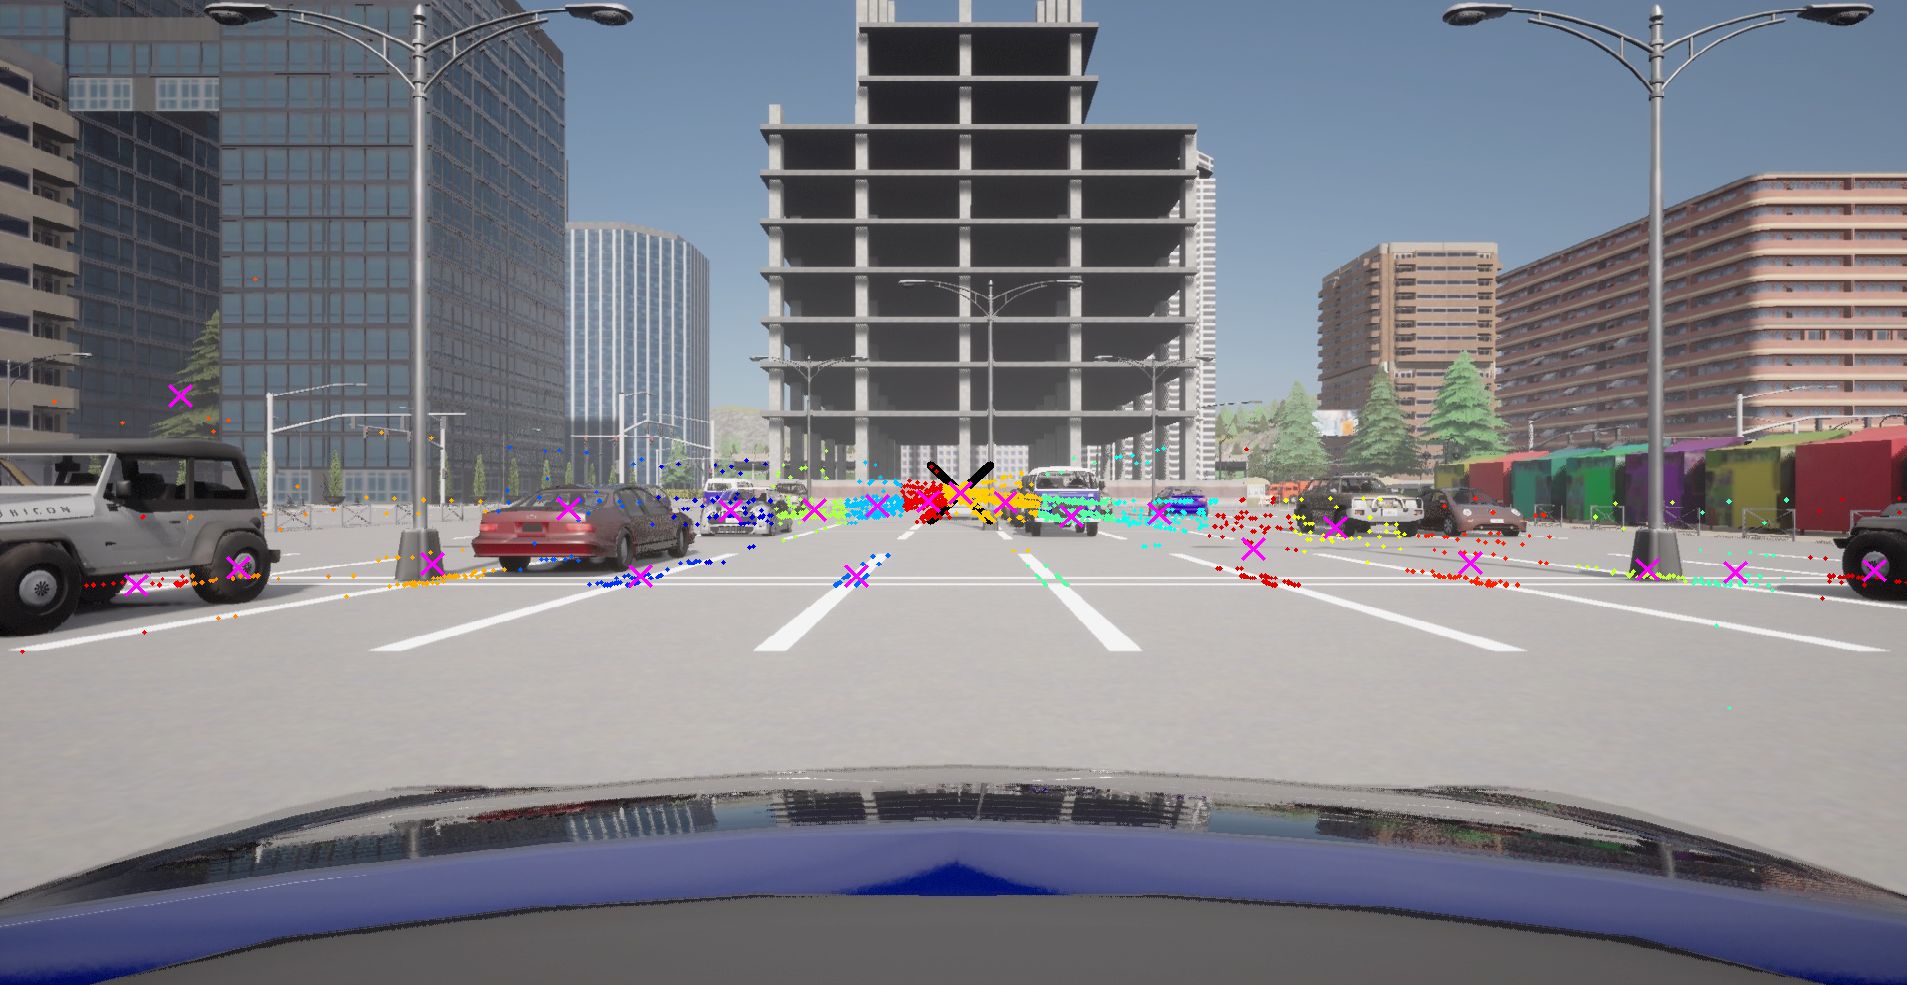
\includegraphics[width=0.8\textwidth]{img/reticule/svd-km}
    \caption{Agrupacion de intersecciones de las líneas detectadas}
    \label{fig:intersections}
\end{figure}

Para estimar la ubicación de este punto de fuga principal no es necesario tener en cuenta todas las intersecciones detectadas,
sino solo aquellas que se encuentran en una zona cercana al horizonte de la imagen.
Esto se debe a que, debido a la perspectiva de la cámara, las líneas paralelas en el mundo real convergen hacia el horizonte en la imagen,
haciendo que los puntos de fuga se ubiquen cerca de esta línea \cite{hartley2003multiple}.
Para determinar las intersecciones relevantes cercanas al horizonte, se puede definir un umbral de cercanía en la imagen que se puede ajustar experimentalmente.
Por ejemplo, en la siguiente imagen se muestran las intersecciones detectadas en la imagen original con puntos azules
y las intersecciones relevantes con un umbral de 10 píxeles con puntos amarillos.
En la figura \ref{fig:relevantInter} se muestra el resultado de la selección de las intersecciones relevantes. \\
\begin{figure}[!ht]
    \centering
    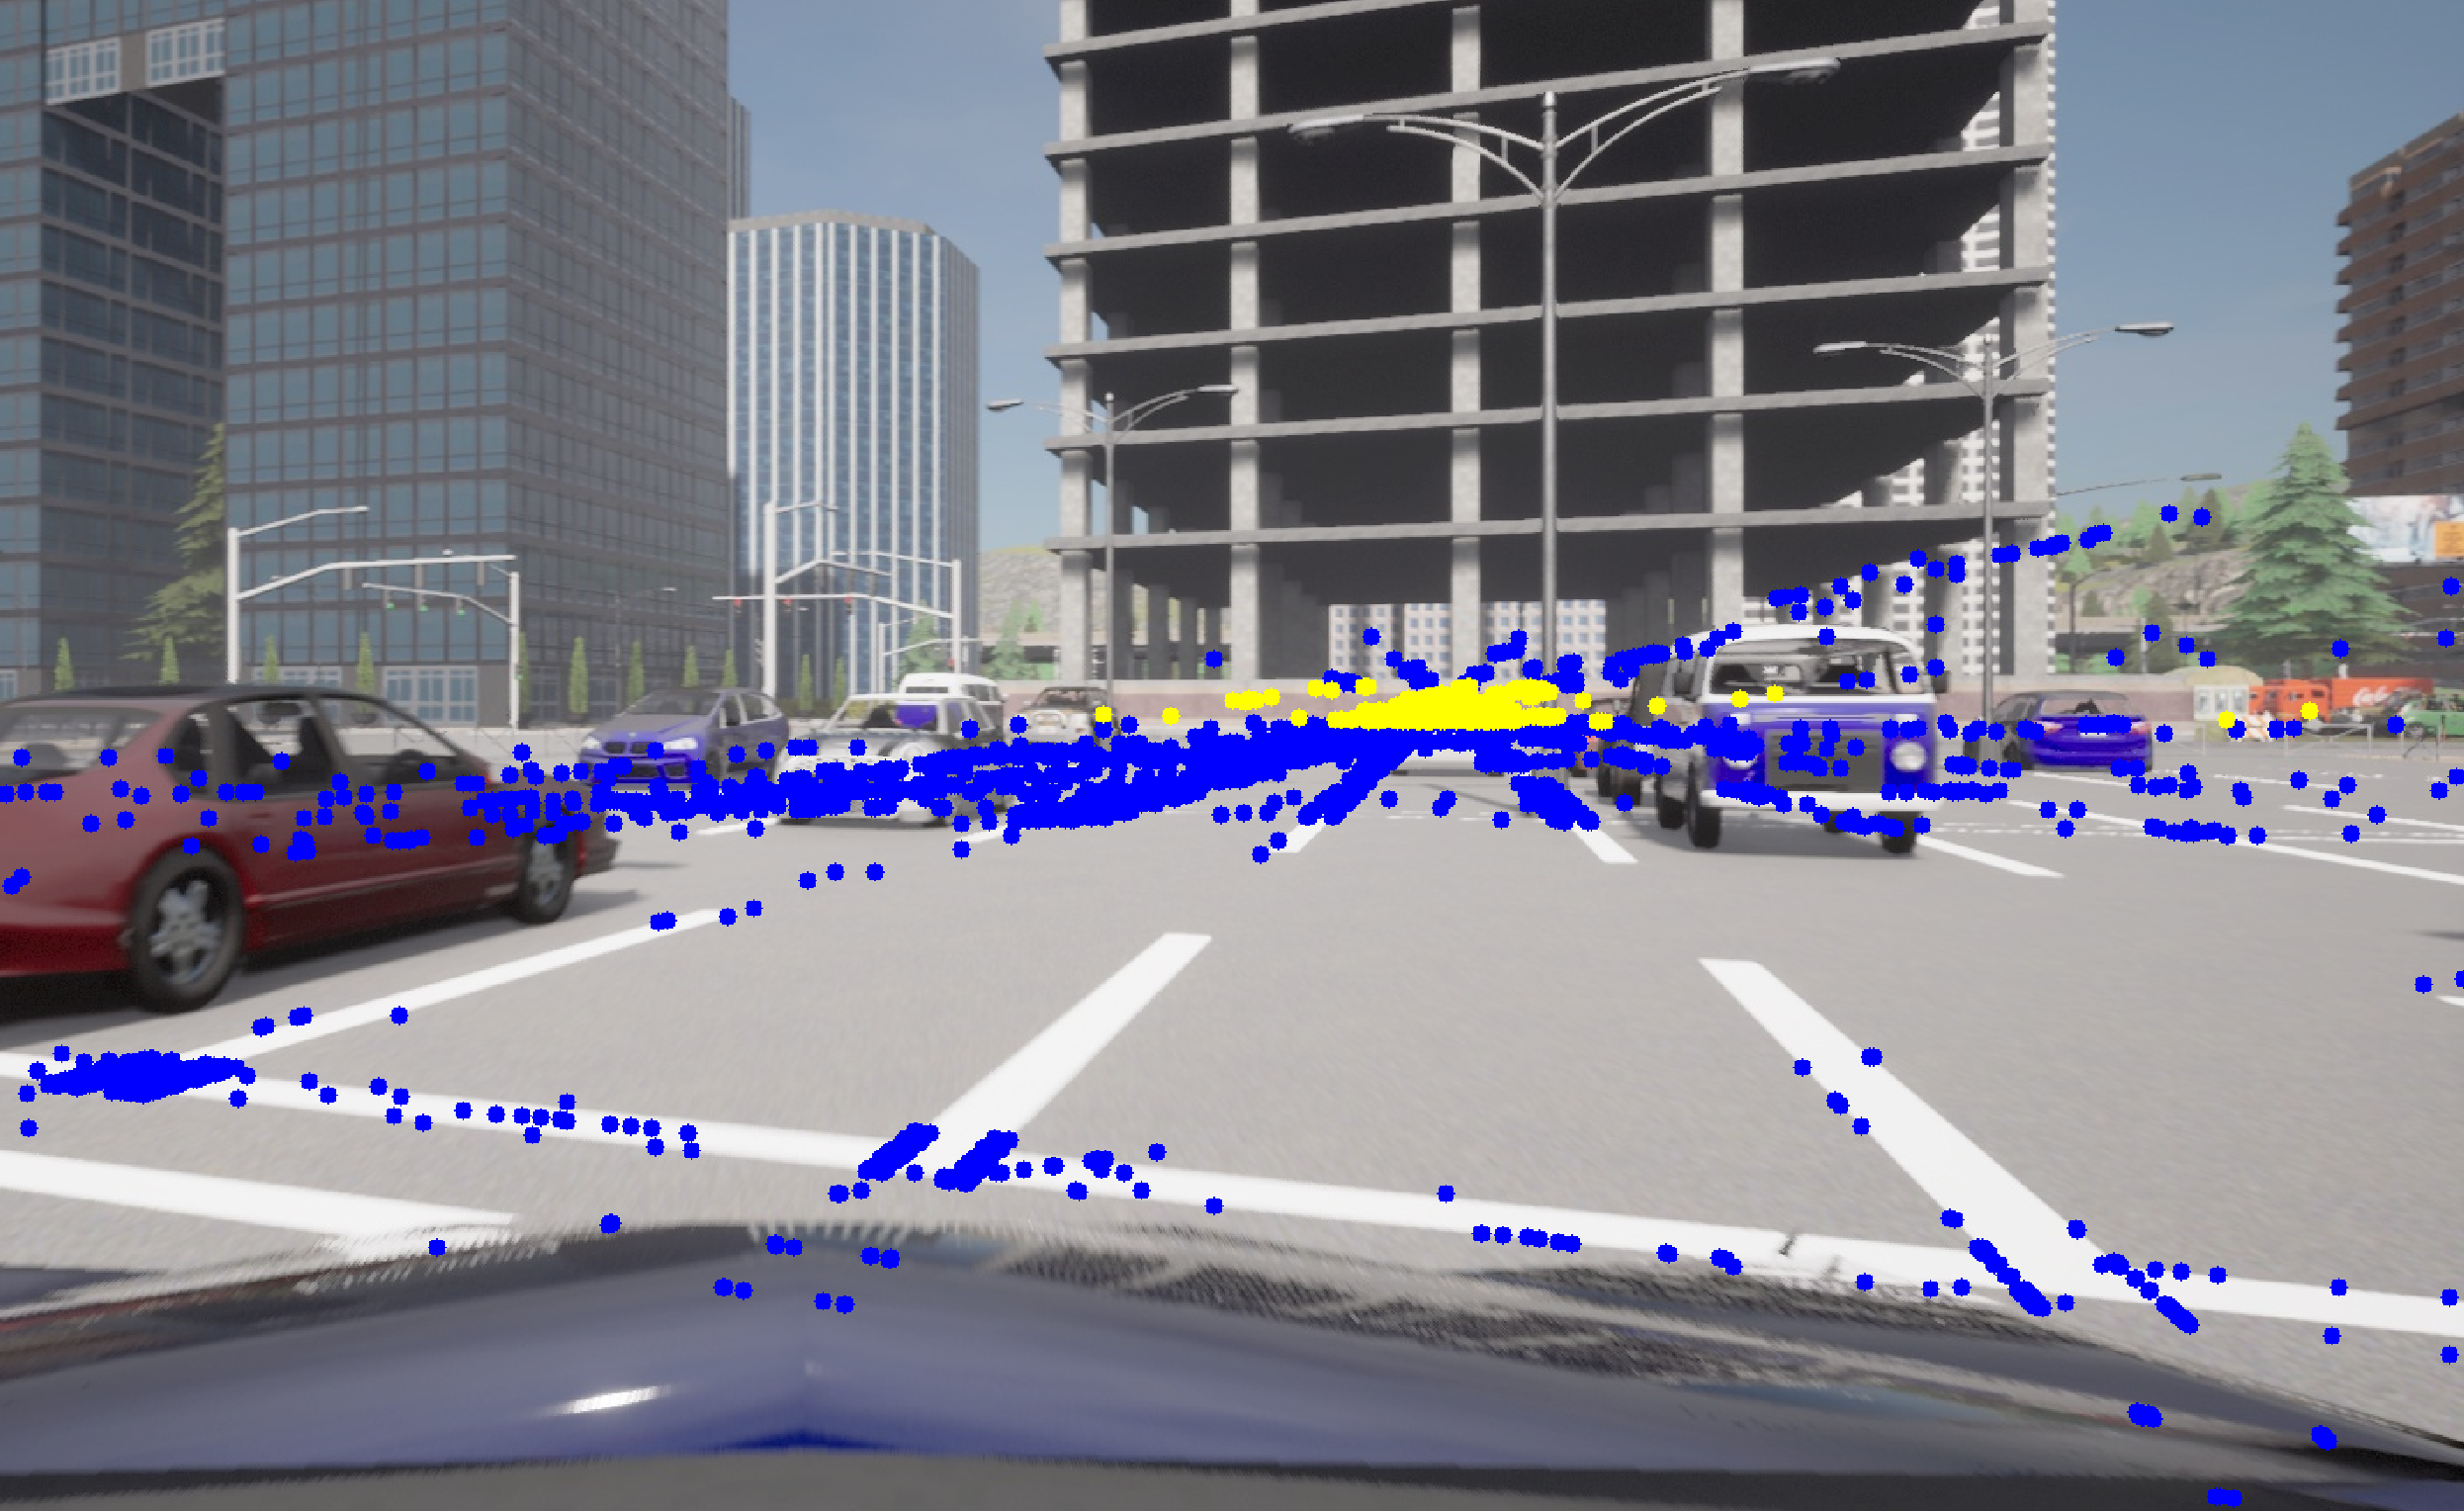
\includegraphics[width=0.8\textwidth]{img/reticule/relevantInter}
    \caption{Intersecciones detectadas en la imagen original}
    \label{fig:relevantInter}
\end{figure}

\textit{Algoritmo de agrupación:}\\

Para realizar la agrupación de las intersecciones relevantes, se utilizó el algoritmo \texttt{AgglomerativeClustering} de la librería \texttt{scikit-learn}.
Este algoritmo fue elegido debido a su capacidad para manejar datos jerárquicos y su flexibilidad para determinar el número óptimo de clusters. Además,
es robusto frente a la variabilidad en la densidad de los puntos de intersección.
El algoritmo de agrupación jerárquica se basa en la idea de que los puntos cercanos entre sí pertenecen al mismo cluster \cite{tan2005introduction}.
Para que el algoritmo determine el número de clusters se utilizó el parámetro \texttt{distance\_threshold}, que indica la distancia máxima
entre dos puntos para que se consideren en el mismo cluster. El valor de este parámetro se puede ajustar experimentalmente.
Por ejemplo, en la siguiente imagen se muestran los mismos puntos de intersección relevantes del ejemplo anterior,
pero agrupados por el algoritmo de agrupación jerárquica en 3 clusters representados de distintos colores, con un símbolo \texttt{+} blanco en el centro de cada cluster.
En la figura \ref{fig:clusters} se muestra el resultado de la agrupación de las intersecciones relevantes.
\begin{figure}[!ht]
    \centering
    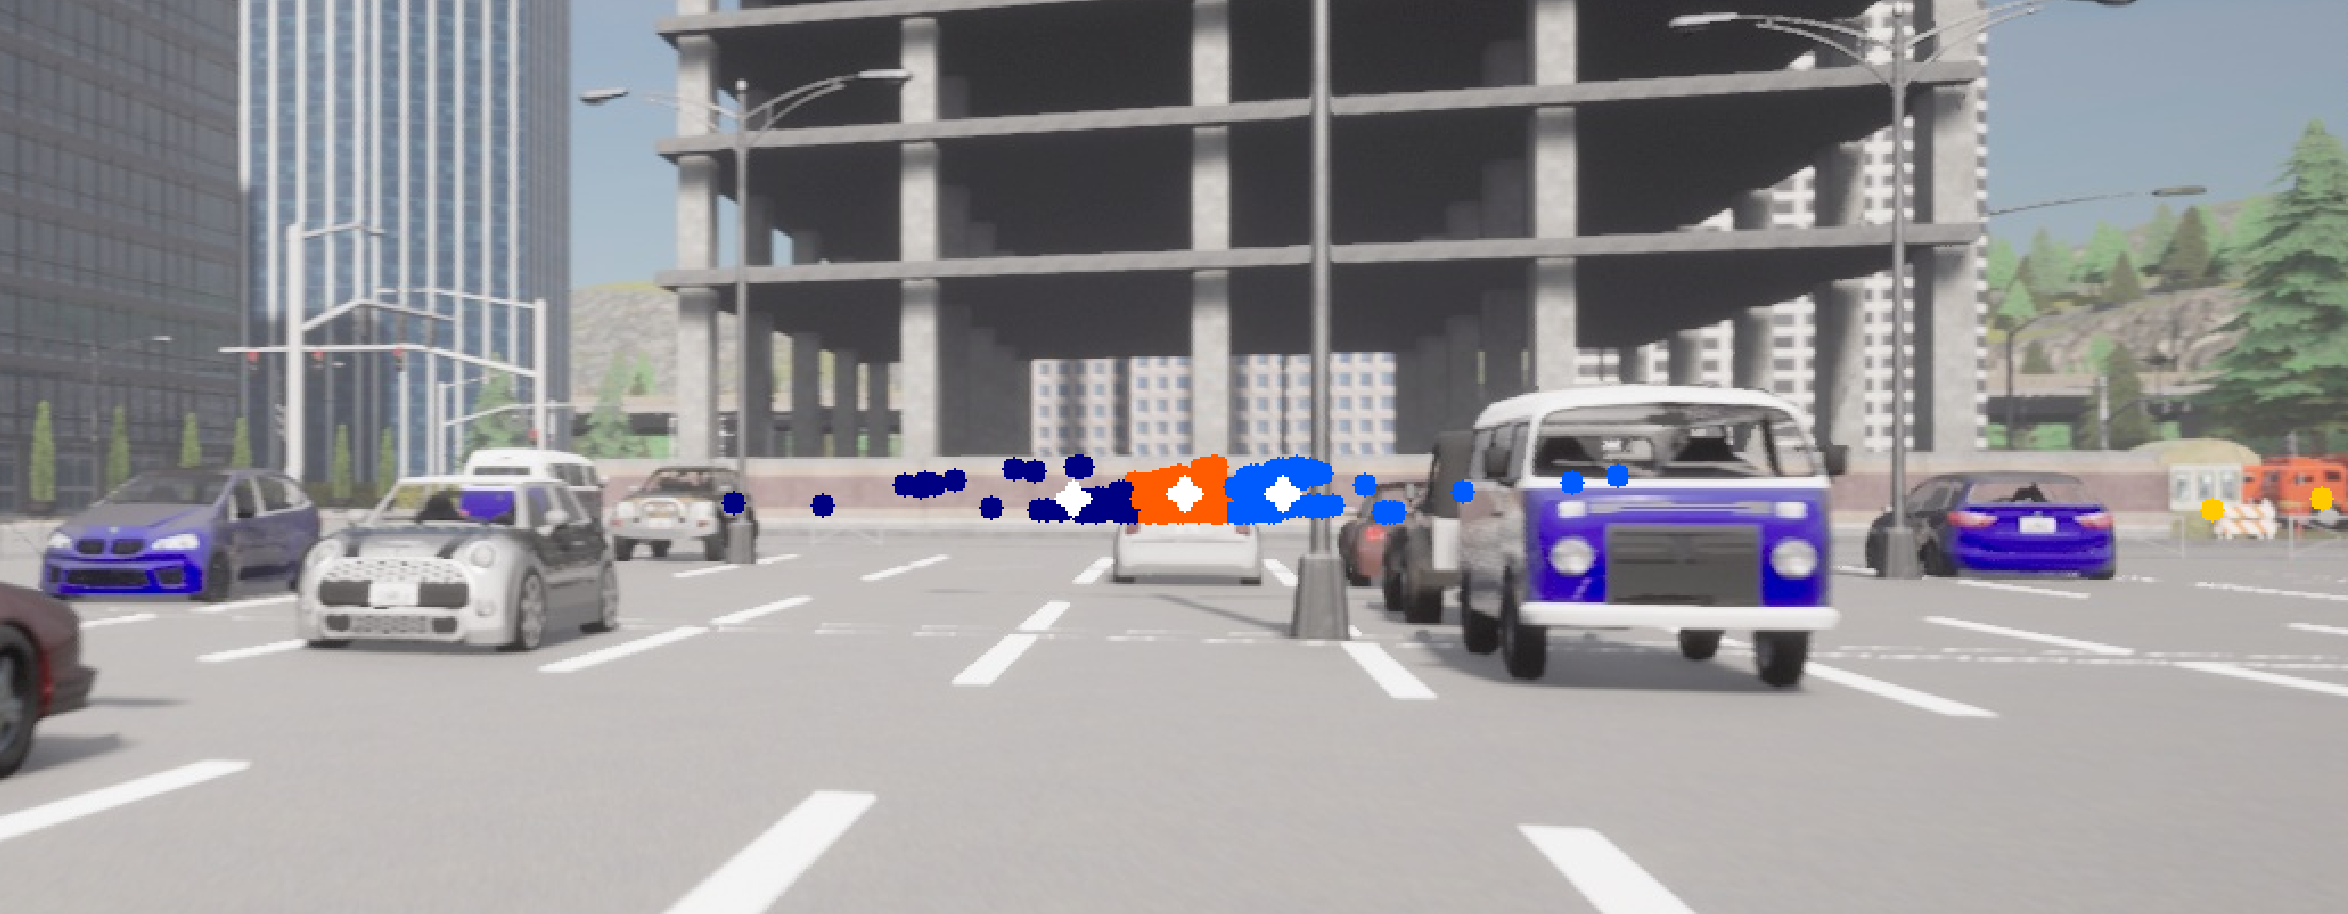
\includegraphics[width=0.8\textwidth]{img/reticule/AgglomerativeClustering}
    \caption{Intersecciones agrupadas en clusters}
    \label{fig:clusters}
\end{figure}



\subsubsection{Selección del punto de fuga principal:}
\noindent
Para estimar la posición del punto de fuga principal, se puede seleccionar el cluster con mayor cantidad de intersecciones y
utilizar las líneas que generaron estos puntos para calcular la intersección de estas líneas.
La intersección de $n$ líneas (bajo un criterio de mínimos cuadrados) está dada por
el eigenvector asociado al eigenvalor más pequeño de la matriz $M$, donde:
\[
    M = \sum_{i=1}^{n} w_i l_i l_i^T
\]
Aquí, $w_i$ es un peso asociado a la línea $l_i$ y $l_i$ es la representación homogénea de la línea $i$ \cite{kanatani1998statistical}.
De esta forma, podemos conocer la posición del punto de fuga principal en el plano de la cámara.
En la figura \ref{fig:vanishingPoint} se muestra el resultado de esta estimación utilizando las líneas del cluster más grande, donde se
representa el punto de fuga principal con un símbolo \texttt{+} amarillo.
\begin{figure}[!ht]
    \centering
    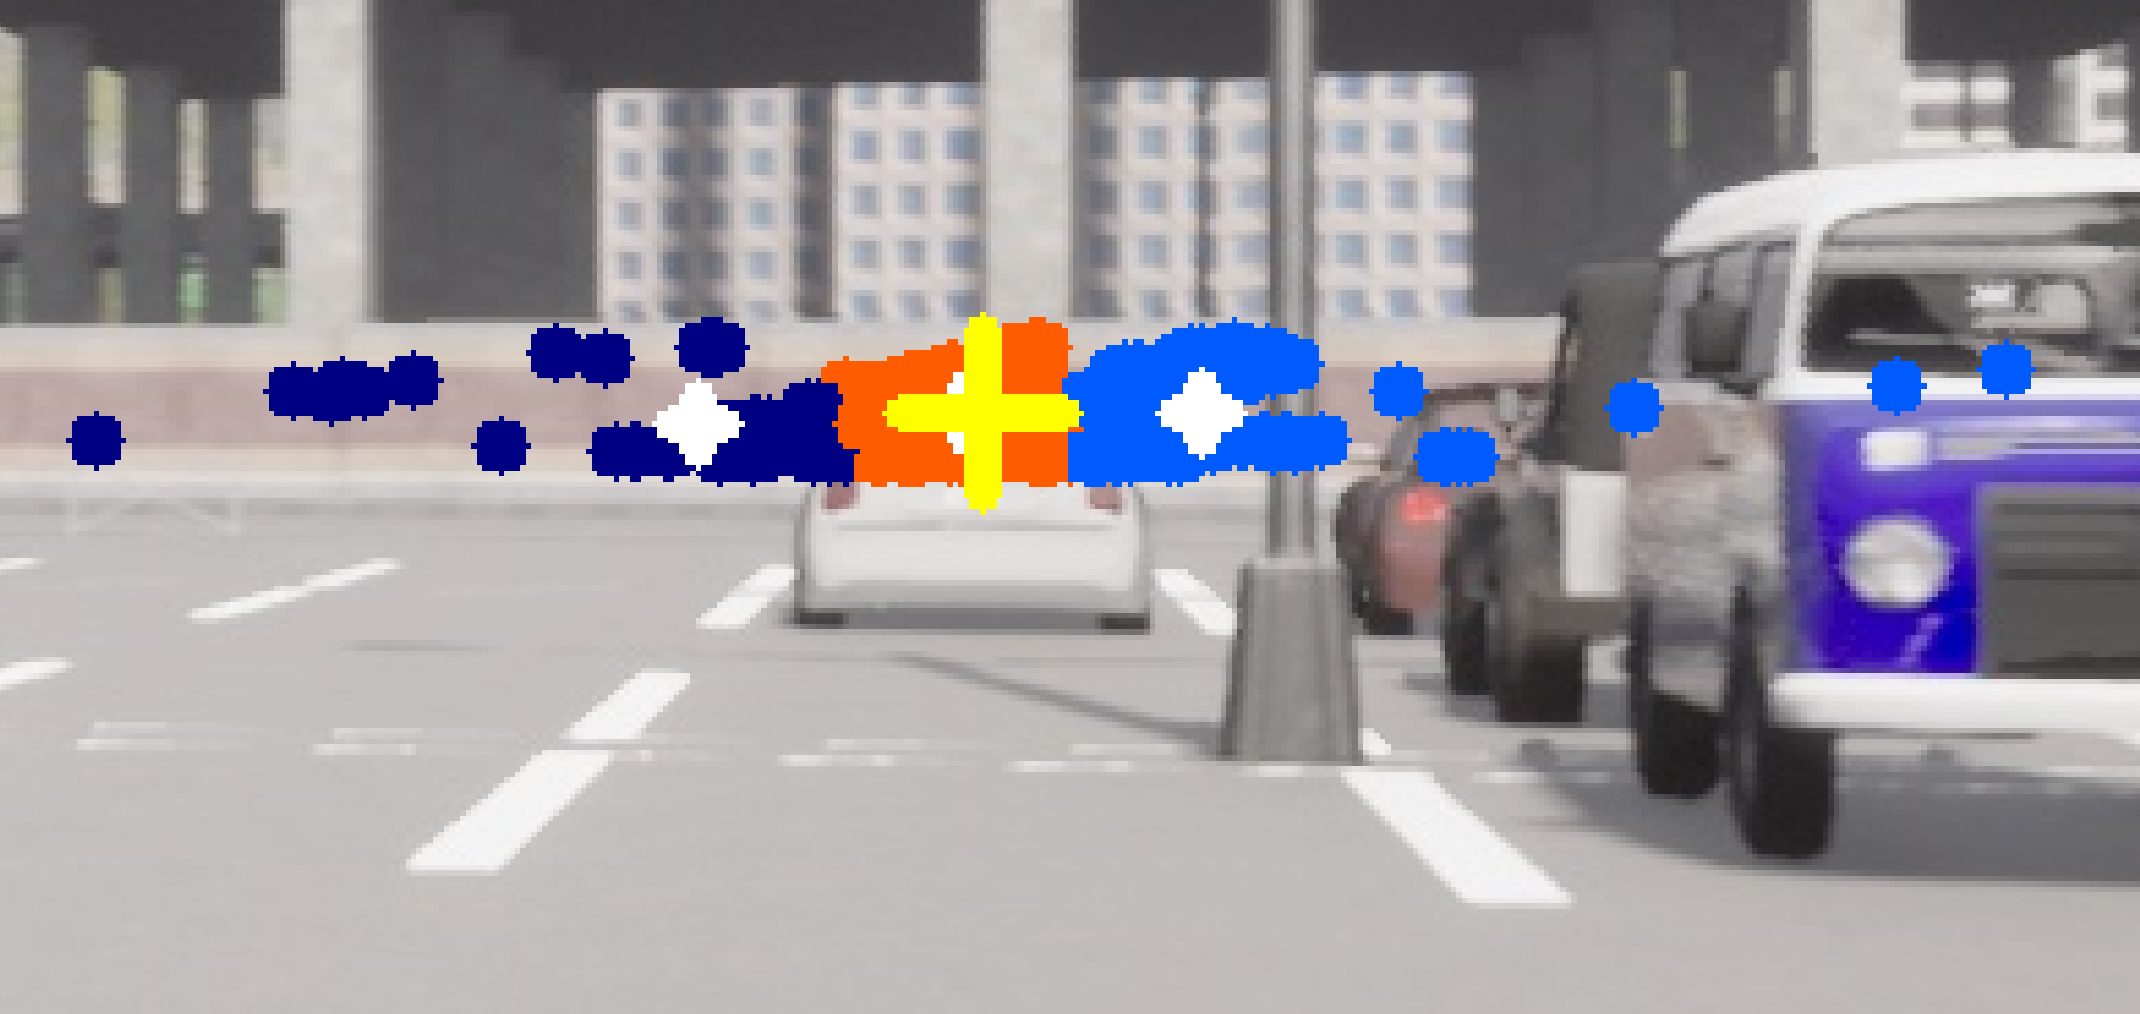
\includegraphics[width=0.8\textwidth]{img/reticule/vanishingPoint}
    \caption{Punto de fuga principal estimado}
    \label{fig:vanishingPoint}
\end{figure}

\subsubsection{Selección del 2do punto de fuga principal:}
Pendiente de redacción.

\subsubsection{Filtrado de intersecciones y líneas relevantes:}
\noindent
Una vez que se han identificado los puntos de fuga principales, se puede proceder a filtrar las intersecciones y las líneas que son
relevantes para la retícula de estacionamiento.
Primero, se filtran las intersecciones que están cerca de los puntos de fuga principales, utilizando un umbral de distancia que se puede ajustar experimentalmente.
Luego, se filtran las líneas que pasan por estas intersecciones relevantes.
Este proceso ayuda a eliminar el ruido y las líneas que no contribuyen a la formación de la retícula de estacionamiento.


\subsubsection{Ajuste de la retícula de estacionamiento utilizando (RANSAC):}
Pendiente de redacción (RANSAC).


\subsubsection{Experimentación y ajuste de parámetros:}\label{subsec:experimentacion-y-ajuste-de-parametros:}
\noindent
Para poder determinar la configuración óptima de los parámetros que se utilizan en los distintos algoritmos de la solución propuesta,
se desarrolló una aplicación en Python que carga una secuencia de imágenes de la trayectoria del vehículo en el estacionamiento y, para cada frame,
calcula la retícula de estacionamiento aplicando los pasos anteriormente descritos.
La aplicación permite visualizar los resultados de cada paso y ajustar dinámicamente los parámetros de los algoritmos para obtener los mejores resultados.
Los parámetros ajustables que se consideraron son:
\begin{itemize}
    \item \texttt{threshold\_image}: Umbral de binarización de la imagen.
    \item \texttt{canny\_threshold\_1}: Umbral inferior para el algoritmo de Canny.
    \item \texttt{canny\_threshold\_2}: Umbral superior para el algoritmo de Canny.
    \item \texttt{hough\_rho}: Resolución de la distancia en píxeles de la cuadrícula de la transformada de Hough.
    \item \texttt{hough\_theta}: Resolución del ángulo en radianes de la cuadrícula de la transformada de Hough.
    \item \texttt{hough\_threshold}: Umbral de votación de la transformada de Hough.
    \item \texttt{hough\_min\_line\_length}: Longitud mínima de la línea en píxeles.
    \item \texttt{hough\_max\_line\_gap}: Máxima separación entre segmentos de línea para tratarlos como una sola línea.
    \item \texttt{relevant\_intersections\_horizon\_threshold}: Umbral de cercanía al horizonte para considerar una intersección relevante.
    \item \texttt{agglomerative\_distance\_threshold}: Distancia máxima entre dos puntos para considerarlos en el mismo cluster.
\end{itemize}
Para analizar el impacto del cambio en los parámetros en tiempo real, la aplicación provee un menú de acciones que permite
representar en la imagen los resultados de cada paso del algoritmo.
%bloque de codigo
%\begin{lstlisting}[language=Python,label={lst:lstlisting22}]
%    --- Leyenda de Teclas ---
%P: Iniciar/Pausar la secuencia de imágenes.
%C: Mostrar/Ocultar contornos.
%L: Mostrar/Ocultar líneas.
%I: Mostrar/Ocultar intersecciones.
%R: Mostrar/Ocultar intersecciones relevantes.
%E: Mostrar/Ocultar líneas relevantes.
%A: Mostrar/Ocultar cúmulos de intersecciones.
%F: Mostrar/Ocultar puntos de fuga.
%G: Mostrar/Ocultar imagen binaria.
%ESC: Salir.
%\end{lstlisting}

\begin{verbatim}
    --- Leyenda de Teclas ---
P: Iniciar/Pausar la secuencia de imágenes.
C: Mostrar/Ocultar contornos.
L: Mostrar/Ocultar líneas.
I: Mostrar/Ocultar intersecciones.
R: Mostrar/Ocultar intersecciones relevantes.
E: Mostrar/Ocultar líneas relevantes.
A: Mostrar/Ocultar cúmulos de intersecciones.
F: Mostrar/Ocultar puntos de fuga.
G: Mostrar/Ocultar imagen binaria.
ESC: Salir.
\end{verbatim}
\noindent
A continuación, en las figuras \ref{fig:experimentationRgb} y \ref{fig:experimentationBinary} se muestra un ejemplo de la aplicación
en ejecución en uno de los frames de la secuencia de imágenes,
donde se visualizan los contornos, las líneas detectadas, las intersecciones, las intersecciones relevantes, las líneas relevantes,
los cúmulos de intersecciones y los puntos de fuga.

\begin{figure}[!ht]
    \begin{subfigure}{0.99\textwidth}
        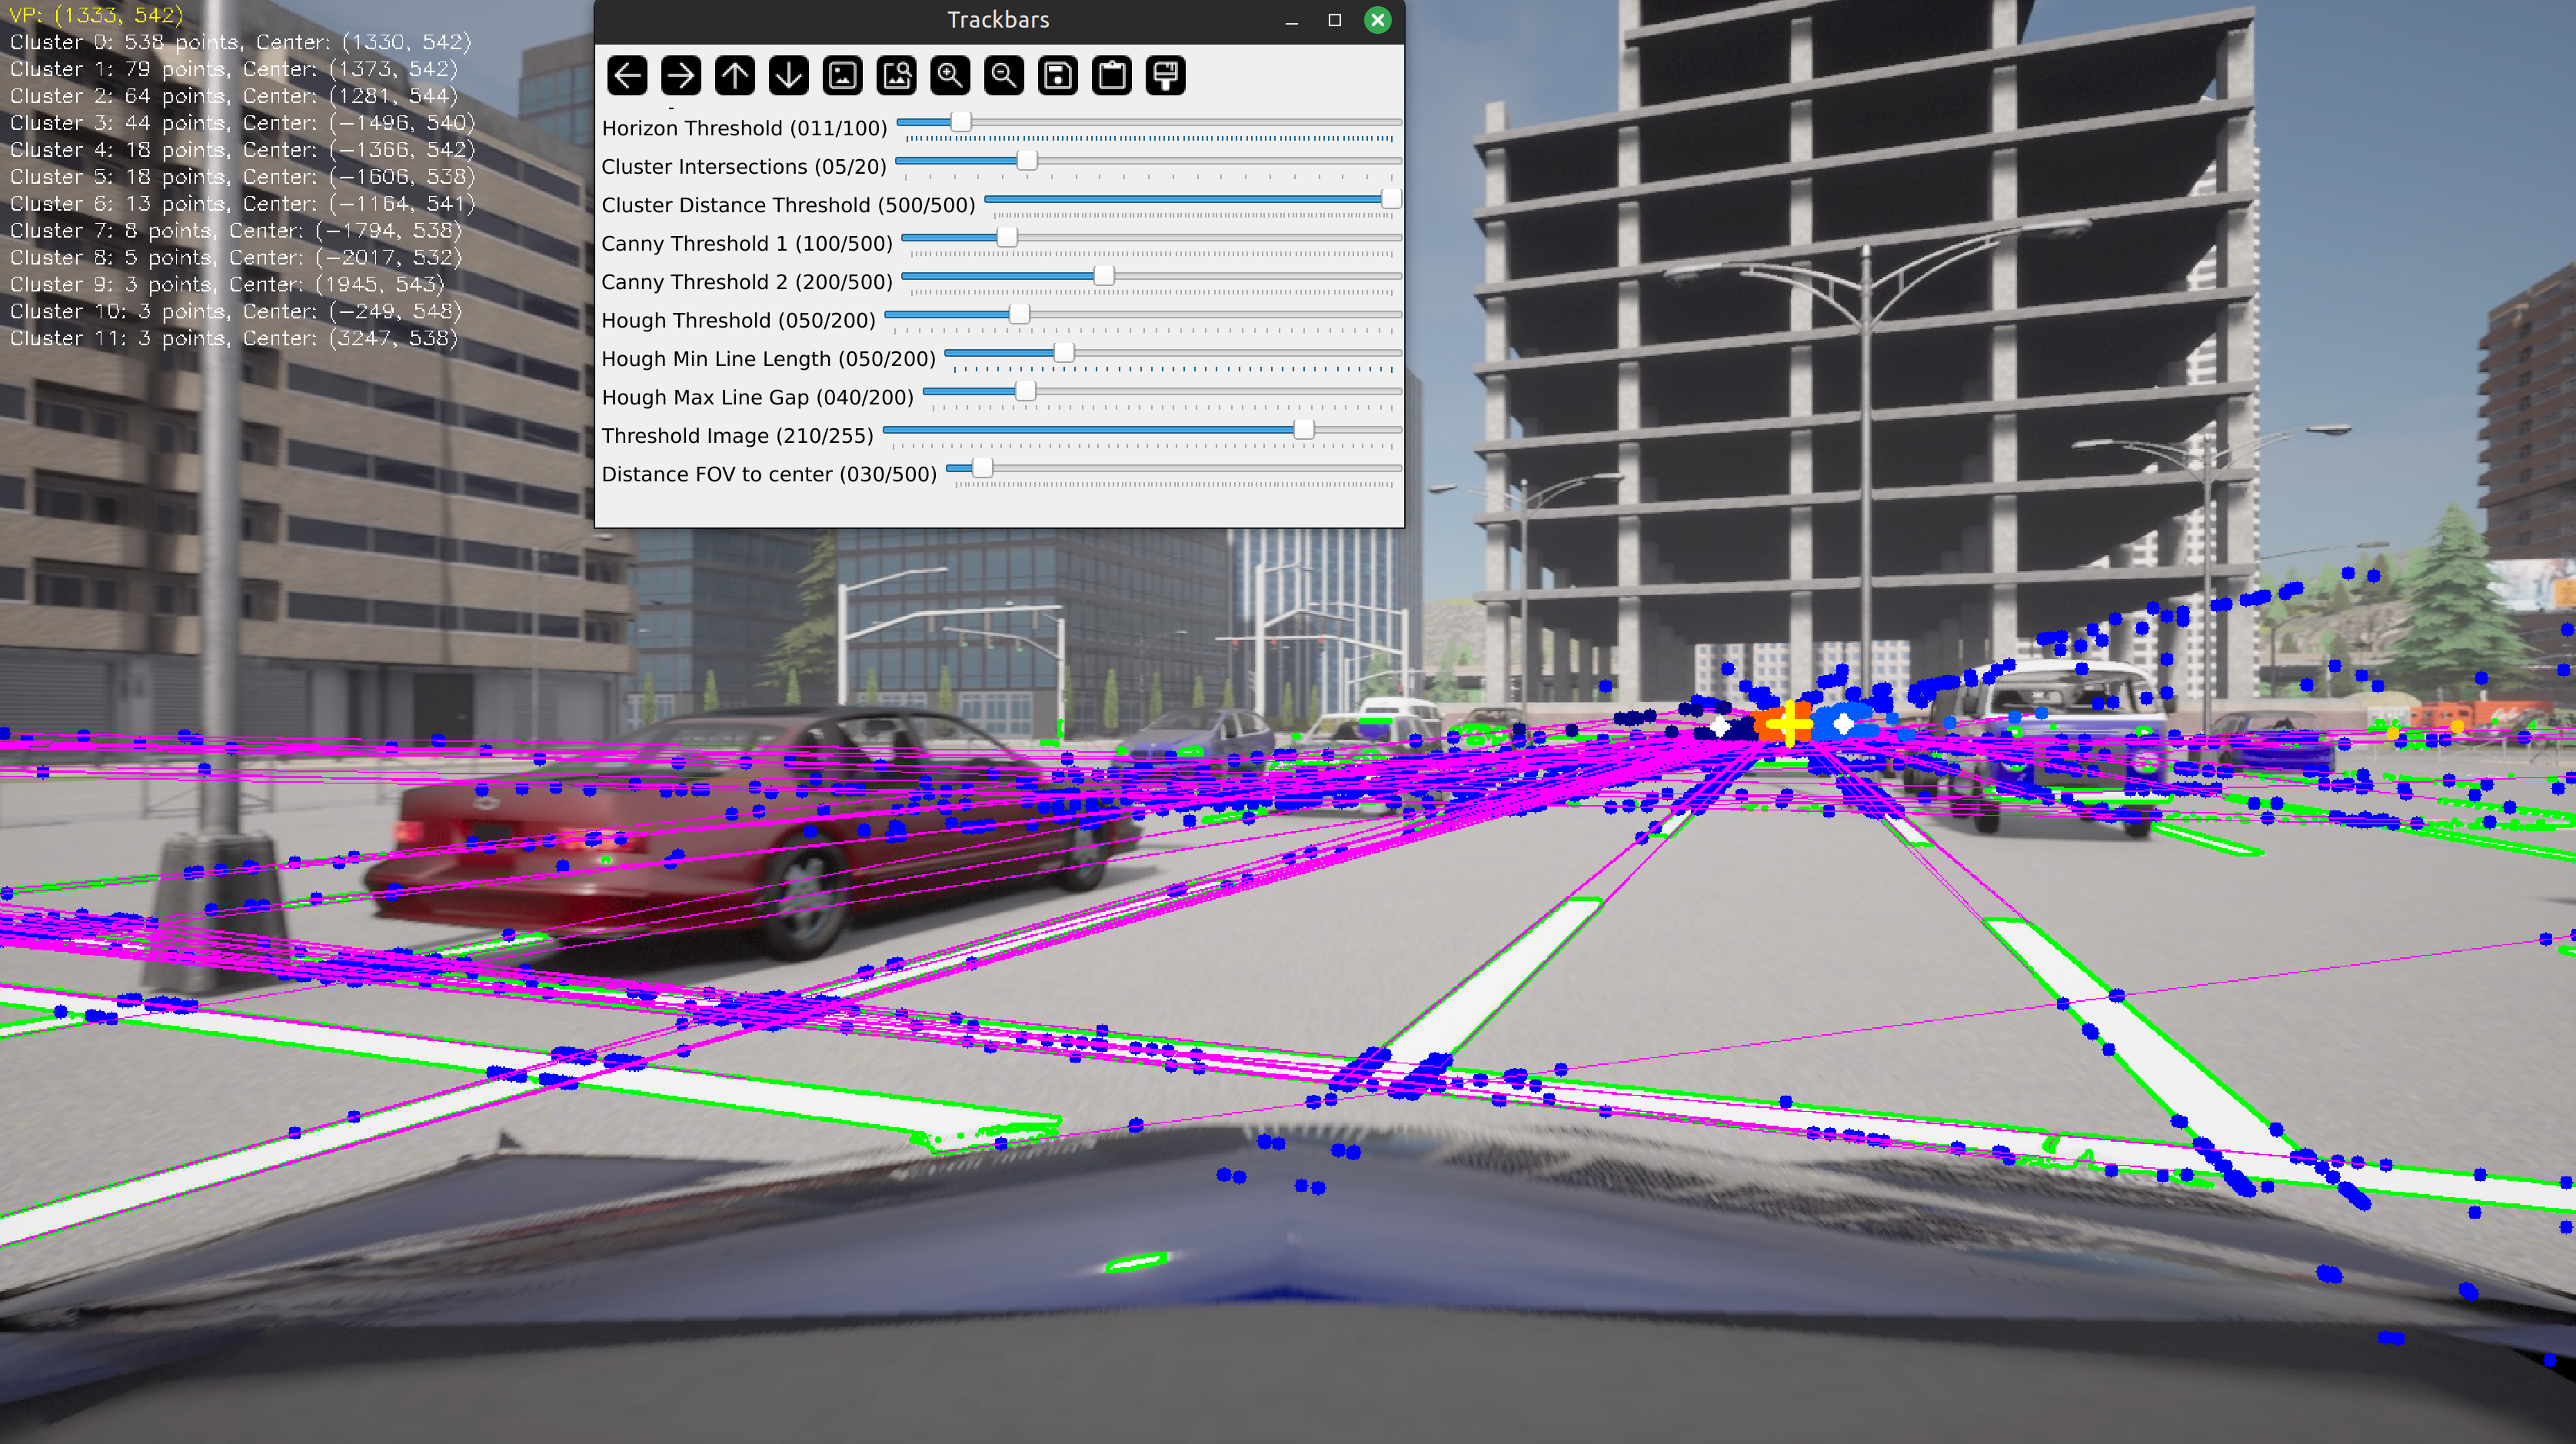
\includegraphics[width=\textwidth]{img/reticule/experimentationRgb}
        \caption{Ejemplo de experimentación (RGB)}
        \label{fig:experimentationRgb}
    \end{subfigure}
    \begin{subfigure}{0.99\textwidth}
        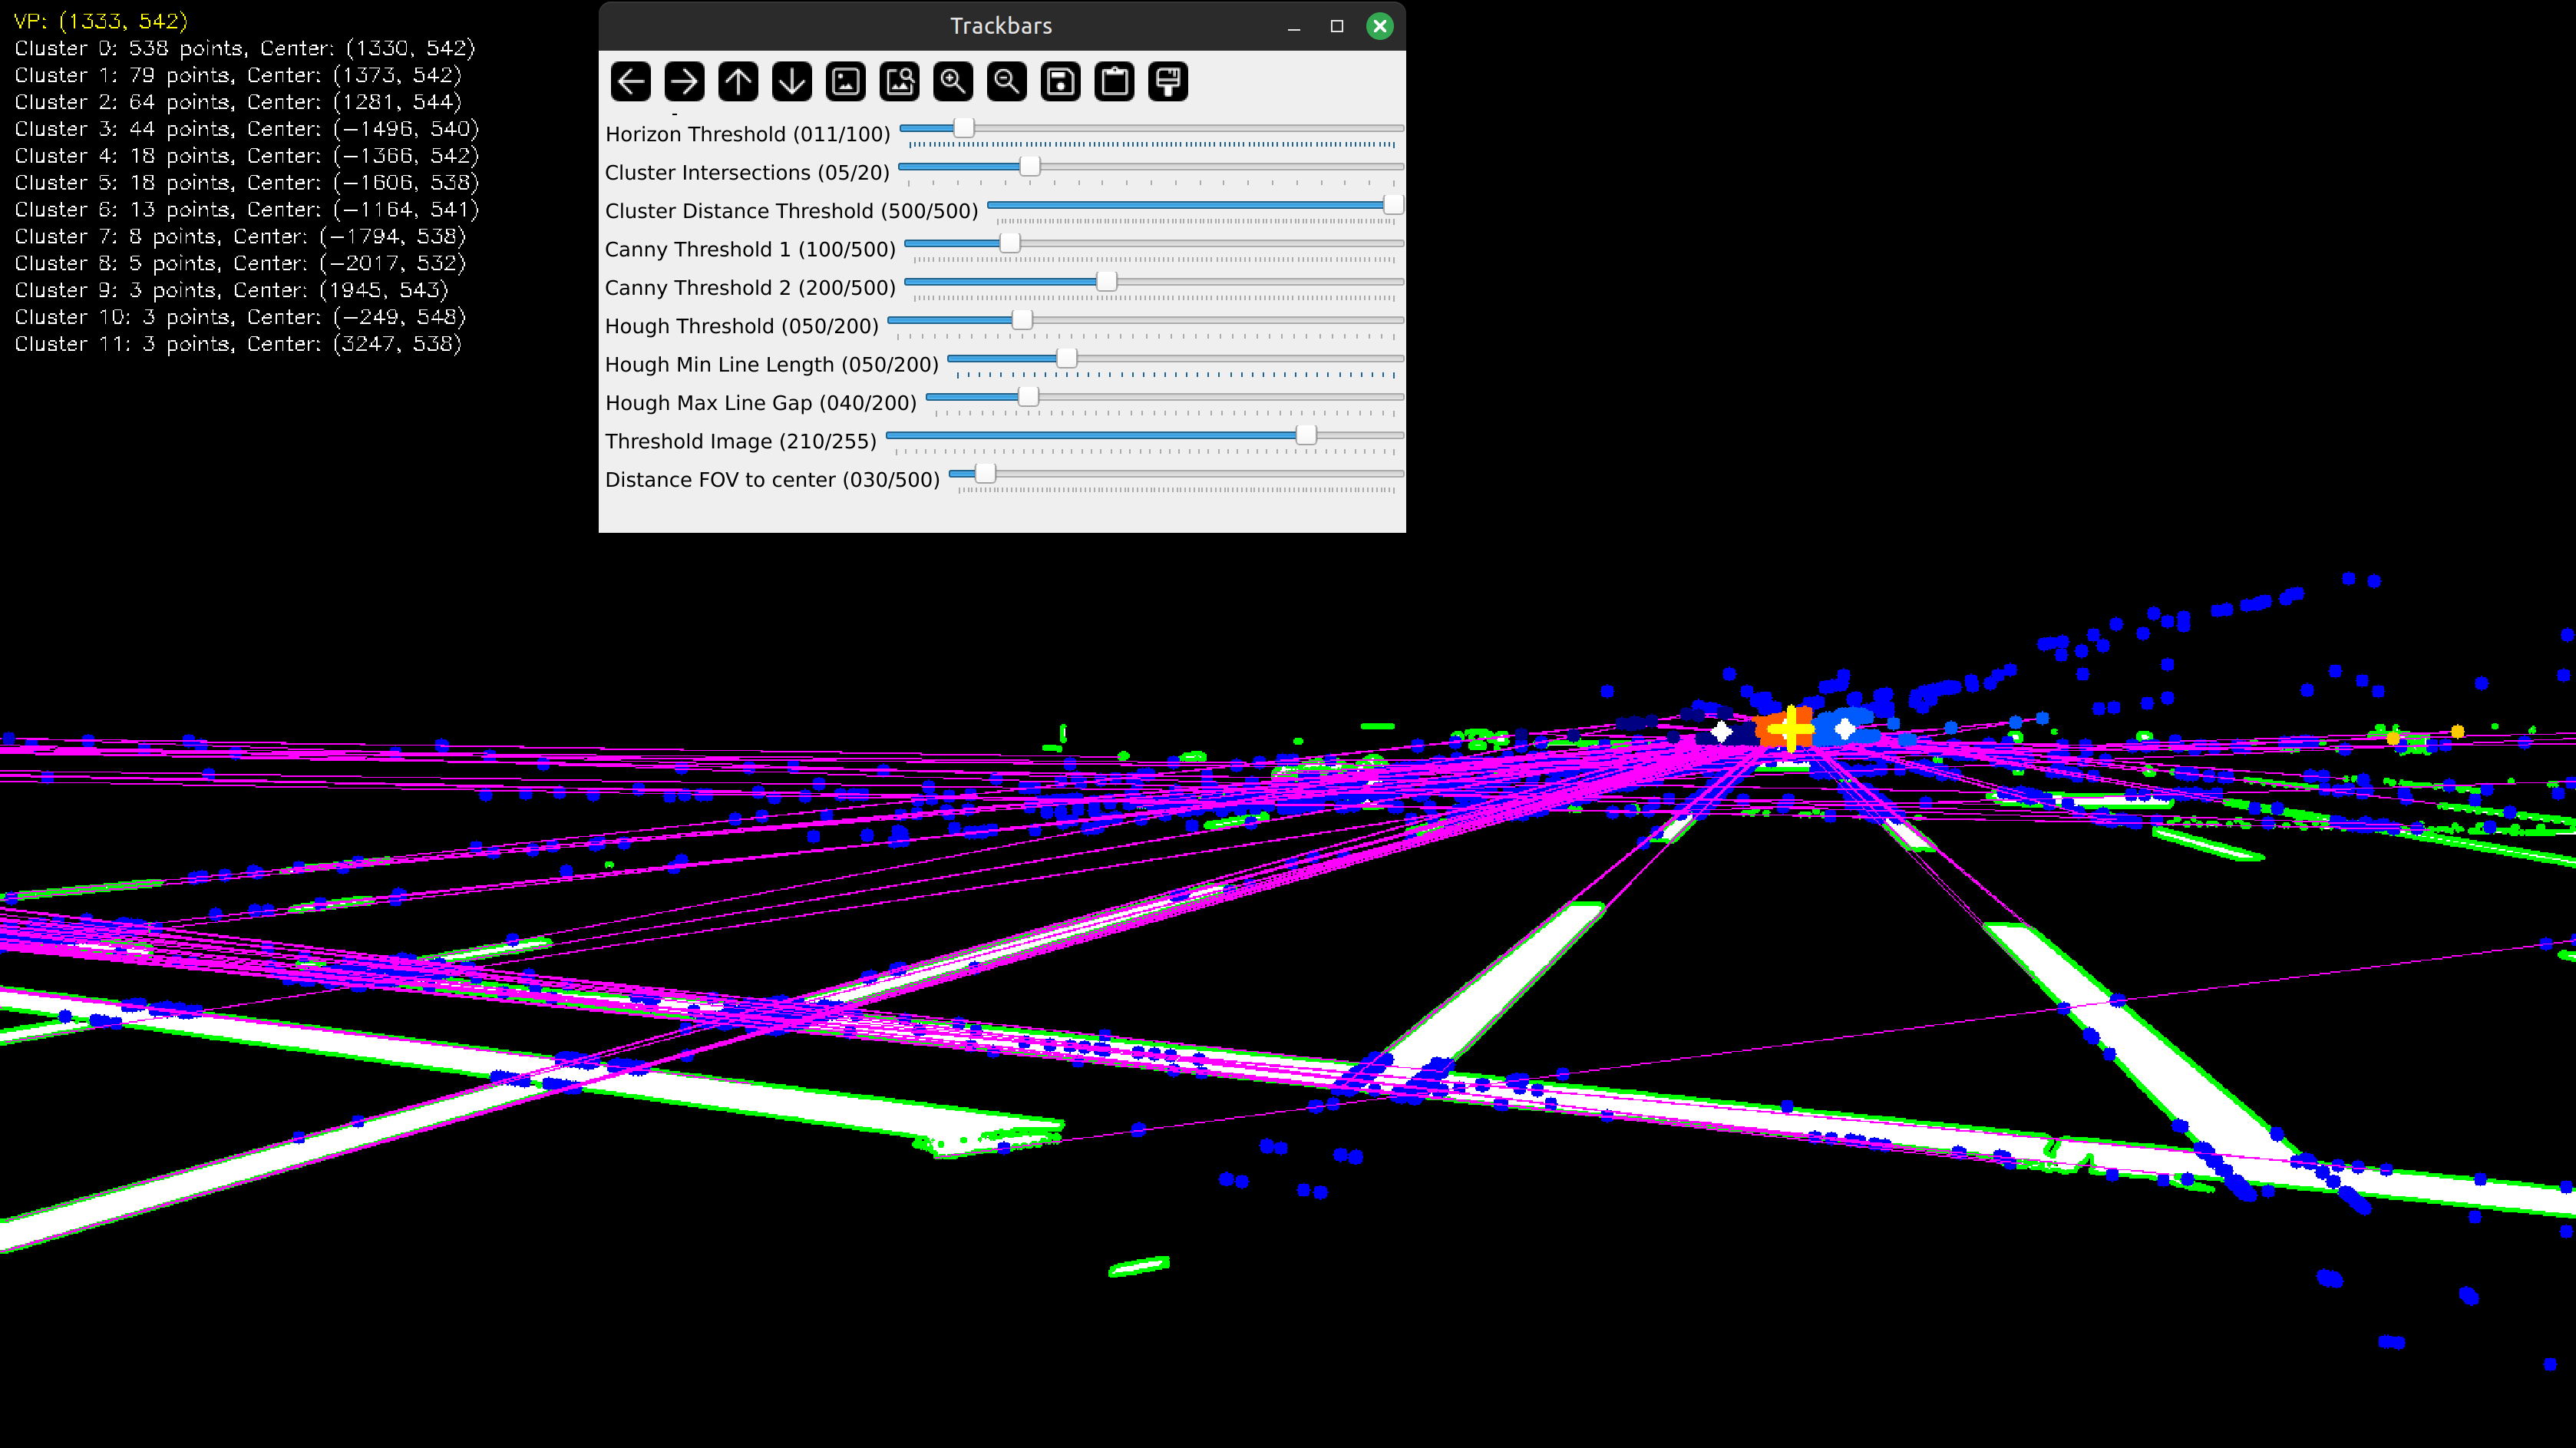
\includegraphics[width=\textwidth]{img/reticule/experimentationBinary}
        \caption{Ejemplo de experimentación (Binaria)}
        \label{fig:experimentationBinary}
    \end{subfigure}
\end{figure}

\noindent
Como se puede observar en la imagen, en el área de Trackbar se muestran los parámetros ajustables y su valor actual,
permitiendo al usuario modificarlos en tiempo real y observar el impacto de estos cambios en la imagen.
Esto facilita la identificación de la configuración óptima para cada parámetro, mejorando la precisión
y la robustez del algoritmo de detección de la retícula de estacionamiento.

\subsubsection{Mediciones en la retícula detectada:}
Pendiente de redacción.


\subsection{Representación de la posición relativa al estacionamiento}
\noindent  Para  representar la  posición  relativa  del vehículo  con
respecto  al espacio  de  estacionamiento, se  propone  un sistema  de
coordenadas cilíndricas en el cual el origen se encuentre en la cámara
del vehículo. Esta elección provee un marco de referencia que facilita
la  medición de  las distancias  y ángulos  necesarios para  maniobrar
adecuadamente  durante   el  estacionamiento.
\noindent Utilizando coordenadas cilíndricas,  es posible describir la
posición  del  vehículo en  términos  de  distancia radial,  ángulo  y
altura, con el origen en la cámara del vehículo permite representar de
manera  directa las  relaciones  espaciales entre  el  vehículo y  los
límites  del espacio  de  estacionamiento. La  altura  conocida de  la
cámara respecto al  suelo proporciona un eje  de referencia constante,
mientras que los ejes orientados  según la dirección y lateralidad del
vehículo facilitan  la interpretación  y cálculo  de la  orientación y
desplazamiento necesarios para estacionar correctamente.

\subsection{Origen del sistema de coordenadas}
Consideramos que el origen del sistema está centrado en la cámara del vehículos, de tal manera que los ejes ortonormales del sistema se definen como sigue:
\begin{itemize}
    \item El eje $z$ se define como un vector unitario en dirección vertical  apuntando hacia el suelo.
    \item El eje $x$ se define como un vector unitario que apunta hacia el frente del vehículo.
    \item El eje $y$ se define como un vector unitario que apunta hacia el lado derecho del vehículo.
\end{itemize}

\begin{figure}[!ht]
    \centering
    \begin{subfigure}{0.4\textwidth}
        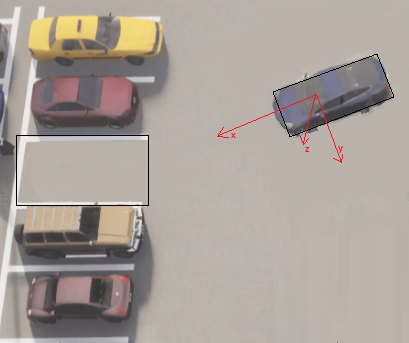
\includegraphics[width=\textwidth]{img/distances_ubi_11}\label {fig:distances11}
    \end{subfigure}
    \begin{subfigure}{0.4\textwidth}
        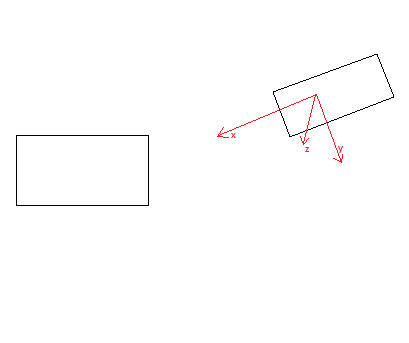
\includegraphics[width=\textwidth]{img/distances_ubi_12}\label {fig:distances12}
    \end{subfigure}
    \caption{Origen del sistema de coordenadas.}
    \label{fig:coord}
\end{figure}
\clearpage

\subsection{Puntos de referencia}
Para representar la posición del vehículo con respecto al espacio de estacionamiento, se establecerán cuatro puntos de referencia:
\begin{itemize}
    \item El punto $1$ se define como la esquina superior izquierda del espacio de estacionamiento.
    \item El punto $2$ se define como la esquina superior derecha del espacio de estacionamiento.
    \item El punto $3$ se define como la esquina inferior izquierda del espacio de estacionamiento.
    \item El punto $4$ se define como la esquina inferior derecha del espacio de estacionamiento.
\end{itemize}
\begin{figure}[!ht]
    \centering
    \begin{subfigure}{0.4\textwidth}
        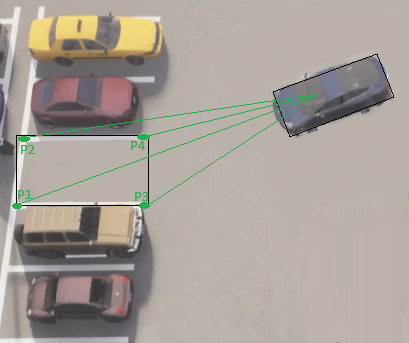
\includegraphics[width=\textwidth]{img/distances_ubi_21}\label {fig:distances21}
    \end{subfigure}
    \begin{subfigure}{0.4\textwidth}
        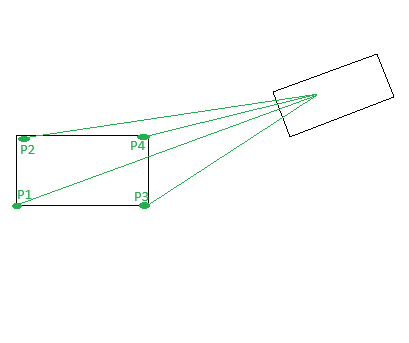
\includegraphics[width=\textwidth]{img/distances_ubi_22}\label {fig:distances22}
    \end{subfigure}
    \caption{Puntos de referencia.}
    \label{fig:coord2}
\end{figure}
\clearpage

\subsection{Coordenadas cilíndricas}
\noindent
Las coordenadas cilíndricas se definen como $(\rho, \theta, z)$, donde:
\begin{itemize}
    \item $\rho$ es la distancia entre el vehículo y un punto de referencia en el espacio de estacionamiento.
    \item $\theta$ es el ángulo de orientación del vehículo con respecto a un punto de referencia en el espacio de estacionamiento.
    \item $z$ es la altura de la cámara con respecto al suelo.
\end{itemize}
\begin{figure}[!ht]
    \centering
    \begin{subfigure}{0.4\textwidth}
        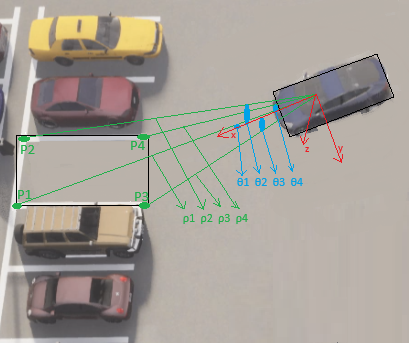
\includegraphics[width=\textwidth]{img/distances_ubi_31}\label {fig:distances31}
    \end{subfigure}
    \begin{subfigure}{0.4\textwidth}
        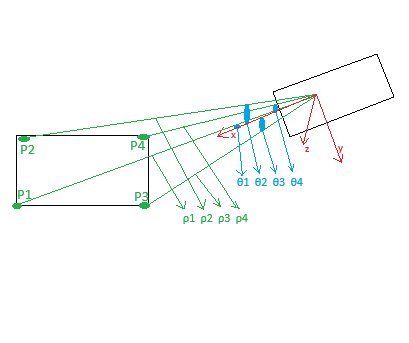
\includegraphics[width=\textwidth]{img/distances_ubi_32}\label {fig:distances32}
    \end{subfigure}
    \caption{Sistema de coordenadas cilíndricas.}
    \label{fig:coord3}
\end{figure}

\subsection{Posición relativa}
La posición relativa del vehículo con respecto al espacio de estacionamiento se representará mediante los 4 vectores de coordenadas cilíndricas:\\
\begin{center}
    $(\rho_1, \theta_1, z)$ , $(\rho_2, \theta_2, z)$ , $(\rho_3, \theta_3, z)$ , $(\rho_4, \theta_4, z)$ \\

\end{center}








% Capítulo 3: Resultados
\clearpage
\section{Resultados}

% Capítulo 4: Conclusiones y trabajo futuro
\clearpage
\section{Conclusiones y trabajo futuro}

% Referencias
\clearpage
\bibliographystyle{acm}
\bibliography{references}

\end{document}